\chapter{Forschungsdesign}

\section{Fragestellungen}

Aus der Forschung geht klar hervor, dass Mädchen und Buben
unterschiedliche Lesepräferenzen haben. Jedoch sind uns keine Studien
bekannt, die das Verhältnis von Leserinnen zu Lesern bei einzelnen
Büchern untersucht haben. Da wir Merkmale von Kinderbüchern mit dem
Geschlecht der Lesenden in Verbindung bringen wollen, ist diese
Information jedoch unabdingbar. Daraus ergibt sich die erste Frage, die
wir in unserer Forschung beantworten wollen.

\begin{frage}\label{fra:andere} Wie schaut das Geschlechterverhältnis\footnote{Unter Geschlechterverhältnis verstehen wir das Verhältnis von weiblichen zu männlichen Personen. In unserem Fall das Verhältnis von Leserinnen zu Lesern.} der Lesenden bei Kinderbüchern aus? \end{frage}

Dabei geht es uns nicht um ein genaues Abbild der Bücher, die gelesen
werden. Vorrangig möchten wir über einige, viel gelesene Bücher das
Geschlechterverhältnis der Lesenden feststellen. Kinderbücher können
anhand mehrerer Kriterien analysiert werden, beispielsweise lassen sie
sich in verschiedene Genres einteilen und Protagonisten können sich ganz
unterschiedlich verhalten. Uns interessiert, ob es Merkmale gibt, die
dafür verantwortlich sind, ob ein Buch bei Mädchen oder Buben beliebter
ist. Daraus ergibt sich die zweite Frage, die wir beantworten möchten.

\begin{frage}\label{fra:unterschiede} Welche inhaltlichen Merkmale von Kinderbüchern hängen mit dem Geschlechterverhältnis zusammen? \end{frage}

Faktoren, die die Leseentscheidung eines Kindes beeinflussen, können
vielfältig sein. Es gibt Faktoren, die keine direkten Merkmale eines
Buchs sind, wie \zB die Beeinflussung durch Gleichaltrige, Geschwister
oder Eltern, Werbung oder Pflichtliteratur in der Schule. Aber es gibt
auch Faktoren, die zu den direkten Merkmalen eines Buchs gehören. Diese
wirken in Situationen, in denen jemand alleine vor einem großen
Bücherregal in einem Bücherei oder einer Bibliothek steht und sich ein
Buch aussucht. Welche Besonderheiten eines Buchumschlages können die
Leseentscheidung beeinflussen? Wir gehen davon aus, dass hier der Inhalt
eine untergeordnete Rolle spielt. Aus dieser Vermutung ergibt sich
unsere dritte Frage.

\begin{frage}\label{fra:merkmale} Kann man, ohne über den Inhalt eines Buchs Bescheid zu wissen, auf das Geschlechterverhältnis der Lesenden schließen? \end{frage}

\section{Hypothesen}

\subsection{Unterschiede im Leseverhalten}

Ausgehend von \thref{fra:andere}, die nach dem Verhältnis von Leserinnen
zu Lesern fragt, interessiert uns, ob wir so etwas wie Mädchenbücher
bzw. Bubenbücher feststellen können. Daraus ergibt sich folgende
Hypothese.

\begin{hyp}\label{hyp:andere}
Mädchen lesen andere Bücher als Buben. Es gibt Bücher, die aufgrund der eindeutigen Bevorzugung eines Geschlechts als Mädchen – oder Bubenbücher bezeichnet werden können. \end{hyp}

\subsection{Eigenschaften der Hauptfigur}

Geschichten erzählen die Handlungen einer Hauptfigur auf eine spezielle
Art und Weise. Zuerst konzentrieren wir uns auf die Hauptfigur an sich.
Viele Studien gehen davon aus, dass sich Leserinnen eher mit weiblichen
und Leser eher mit männlichen Hauptfiguren identifizieren. Wir wollen
überprüfen, ob sich das auch so im Leseverhalten der Kinder
widerspiegelt. Daraus ergeben sich folgende Hypothesen:

\begin{hyp}\label{h2} Es gibt einen Zusammenhang zwischen dem Geschlecht der Hauptfigur und dem Geschlecht der Lesenden. \end{hyp}

\begin{subhyp}\label{h2.1} Ist die Hauptfigur weiblich, wird ein Buch bevorzugt von Mädchen gelesen. \end{subhyp}

\begin{subhyp}\label{h2.2} Ist die Hauptfigur männlich, wird ein Buch bevorzugt von Buben gelsen. \end{subhyp}

Bis jetzt haben wir uns am Geschlecht der Hauptfigur orientiert, aber
wir möchten ebenso etwas über ihr Gender erfahren, weil wir vermuten,
dass Mädchen eher über feminine und Buben über maskuline Protagonisten
lesen, unabhängig davon, ob diese weiblich oder männlich
sind.\footnote{Wenn die Begriffe weiblich und männlich in dieser Arbeit verwendet werden, weisen sie auf das Geschlecht hin, die Begriffe feminin und maskulin stehen für Gendereigenschaften.}

\begin{hyp}\label{h3} Es gibt einen Zusammenhang zwischen dem Geschlechterverhältnis der Lesenden und dem Verhältnis von femininen und maskulinen Verhaltenseigenschaften der Hauptfigur. \end{hyp}

\begin{subhyp}\label{h3.1} 
  Umso femininer sich die Hauptfiguren verhalten, desto höher ist der Anteil an Leserinnen.\end{subhyp}

\begin{subhyp}\label{h3.2} Je maskuliner Protagonisten dargestellt werden, desto eher handelt es sich um eine vorwiegend männliche Leserschaft.\end{subhyp}

\subsection{Inhaltliche Merkmale von Geschichten}

Wir haben uns in einem ersten Schritt auf Themen konzentriert und
vermuten, dass Geschichten, die sich um Pferde, Prinzessinnen oder Hexen
drehen, hauptsächlich von Mädchen bevorzugt werden. Geschichten über
Fußball, Bösewichte, Drachen oder Indianer sprechen Buben stärker an als
Mädchen.

\begin{hyp}\label{hyp:themen} Mädchen und Buben interessieren sich für unterschiedliche Themen. \end{hyp}

In einem zweiten Schritt untersuchen wir wesentliche Aspekte der
Geschichten. Zuerst soll geprüft werden, ob es sich um eine Abenteurer-
oder Alltagsgeschichte handelt. Wir gehen davon aus, dass Buben eher
Abenteuergeschichten lesen und Alltagsgeschichten von Mädchen bevorzugt
werden.

\begin{subhyp}\label{h4.1} Abenteuergeschichten werden eher von Buben als von Mädchen gelesen. \end{subhyp}

In vielen Abenteuergeschichten geht es darum, bestimmte Fälle zu lösen.
Doch es gibt auch Alltagsgeschichten, in denen bestimmte Aufgaben gelöst
werden müssen. Aus diesem Grund überprüfen wir separat, ob es in
Geschichten um das Lösen von Quests geht. Wir gehen davon aus, dass
solche zielgerichteten Geschichten eher von Buben gelesen werden.

\begin{subhyp}\label{h4.2} Geschichten in denen \emph{Quests} vorkommen werden eher von Buben als von Mädchen gelesen. \end{subhyp}

Der nächste Aspekt, dem wir uns zuwenden, ist der Innere Monolog. Können
wir im Buch etwas über die Gedanken, Gefühle, die psychischen Innenwelt
der Hauptfigur erfahren? Wir wollen überprüfen ob Geschichten, in denen
diese Elemente charakteristisch sind, bei Mädchen beliebter sind.

\begin{subhyp}\label{h4.3} Geschichten, in denen ein \emph{Innerer Monolog} vorkommt, werden eher von Mädchen gelesen als von Buben. \end{subhyp}

Es gibt Kindergeschichten, in denen die Hauptfigur bleiben darf wie sie
ist. In anderen Geschichten ist das Erwachsenwerden der Figur relevant.
In diesen Geschichten muss sich der Protagonist verändern, anpassen und
lernen sich nach bestimmten Regeln zu verhalten.

\begin{subhyp}\label{h4.4} Geschichten, in denen \emph{das Erwachsenwerden} Thema ist, werden eher von Mädchen als von Buben gelesen. \end{subhyp}

\begin{subhyp}\label{h4.5} Wenn phantastische Elemente in Geschichten vorkommen, ist der Anteil der Leserinnen größer als der der Leser.
\end{subhyp}

Ein stereotypes Attribut des weiblichen Geschlechts ist Verträumtheit,
im Gegensatz dazu steht Rationalität und realistisches Denken, welche(s)
eher Männern zugerechnet wird. Wir vermuten, dass Mädchen eher von
phantastischen Elementen fasziniert sind als Buben.

\subsection{Oberflächliche Merkmale der Bücher}

In \thref{fra:merkmale} haben wir gefragt, ob man von äußeren Merkmalen
eines Buchs, auf das Geschlechterverhältnis der Lesenden schließen kann,
ohne den Inhalt zu kennen.

\begin{hyp}\label{h5} Man kann das Geschlechterverhältnis rein durch äußerliche Merkmale eines Buchs erklären. \end{hyp}

\begin{subhyp}\label{h5.1} Wenn ein Buchumschlag hell gestaltet ist, sollen Mädchen angesprochen werden. Wir vermuten, dass dunkle Büchern umgekehrt auf eine vorwiegend männliche Leserschaft schließen lassen.\end{subhyp}

\begin{subhyp}\label{h5.2} Wenn im Titel eines Buchs ein weiblicher Name vorkommt oder eine weibliche Figur am Cover abgebildet ist, spricht dieser Titel eher Mädchen an.\end{subhyp}

Wir wollen herausfinden ob Bubenbücher mehr Titelfiguren haben als
Mädchenbücher, da wir aus der Literatur wissen, dass Buben häufiger in
Gruppen, während Mädchen eher mit der besten Freundin spielen.

\begin{subhyp}\label{h5.3} Autorinnen schreiben eher Bücher für Mädchen; Autoren haben tendenziell ein eher männliches Lesepublikum.\end{subhyp}

\begin{subhyp}\label{h5.4} Je dicker ein Buch ist, desto eher wird es von Mädchen gelesen.\end{subhyp}

In der Literatur wird immer wieder darauf hingewiesen, dass Buben
weniger lesen als Mädchen und deshalb auch weniger geübt und langsamer
bei diser Tätigkeit sind.

\section{Methoden}

\subsection{Fragebogenerhebung}

Um \thref{hyp:andere} zu testen, müssen wir zuerst herausfinden, welche
Bücher von welchem Geschlecht gelesen werden. Dafür möchten wir Kinder
der 3. und 4. Schulstufe (8-10 Jahre) befragen, welche Bücher sie
bereits gelesen haben. Wir haben uns entschieden, den Kindern eine Liste
von Büchern vorzulegen, bei denen sie nur noch Ankreuzen müssen. Die
Liste der Bücher erstellen wir anhand von Bestsellerlisten, der Analyse
von Verleihdaten einer Schulbibliothek und dem Gespräch mit
Volksschullehrerinnen und einer Büchereimitarbeiterin. Zusätzlich bieten
wir eine, der Liste vorangestellte, offene Frage an, die nach den
Lieblingsbüchern der Kinder fragt. Außerdem gibt es noch eine Liste von
Themen, die angekreuzt werden können. Bei der Auswahl der Volksschulen
achten wir darauf, möglichst viele verschiedenen Milieus abzudecken. Es
sollen insgesamt 500 Kinder befragt werden. Mit einem
$\chi^2$-Vierfeldertest stellen wir für jedes Buch, das insgesamt mehr
als 50 Nennungen hat, fest ob ein signifikanter Unterschied zwischen der
Anzahl der Leserinnen und der Anzahl der Leser besteht. Danach können
wir \thref{hyp:andere} beantworten. Für \thref{hyp:themen} gehen wir
gleich vor und testen, ob das Geschlecht das Interesse für bestimmte
Themen beeinflusst. Wir benötigen einen Wert, der das
Geschlechterverhältnis der Lesenden angibt. Dafür bilden wir eine Skala,
die von $-1$ bis $1$ geht. $-1$ heißt, dass ein Buch nur von Mädchen
gelesen wird. $1$ heißt, dass ein Buch nur von Buben gelesen wird. Mit
Hilfe dieser Skala wird ein Faktor, der w/m-Faktor, wie folgt gebildet.

\begin{equation} w/m=\frac{Buben-Mädchen}{Mädchen+Buben} \end{equation}

\subsection{Inhaltsanalyse}

Die nächsten Hypothesen beschäftigen sich mit der Hauptfigur. Wie
bereits im Literaturteil erwähnt, gehen wir davon aus, dass jede
Geschichte eine Hauptfigur hat. Es kann sich dabei auch um einen
Pluralprotagonisten, wie \zB eine Bande handeln. Das Geschlecht des
Protagonisten kann entweder eindeutig weiblich, männlich oder unbestimmt
sein. Für \thref{h2} modellieren wir wieder eine lineare Multiple
Regression, wobei das Geschlecht der Hauptfigur in Dummy-Variablen
umkodiert werden muss. Für \thref{h2.1} und \thref{h2.2} berechnen wir
eine Korrelation dem Geschlecht der Hauptfigur (hier wurde nur männlich
und weiblich berücksichtigt) und dem w/m-Faktor. Für \thref{h3}
benötigen wir ein Merkmal, dass das Verhalten der Hauptfigur beschreibt,
und zwar im Hinblick auf feminine oder maskuline
Verhaltenseigenschaften. Um das Verhalten der Hauptfigur zu messen,
bilden wir anhand einer Tabelle von geschlechterstereotypen
Gegensatzpaaren ein semantisches Differenzial.
\parencites[174\psq]{feldmann2006}[93\psqq]{Spillner1974} Jeder
Hauptfigur sollen Extremwerte zugeordnet werden. Um die Güte der
Codierung zu überprüfen, wird jede Hauptfigur von zwei Personen codiert
und die Ergebnisse gegenseitig kontrolliert.



      \ctable[
      %  cap    = ,
        caption = {Geschlechterstereotype},
        label   = stereo ,
        % pos   = htp,
      %  width    = \textwidth
      ]{ll}{
        \tnote{Quelle: \inparencite[175]{feldmann2006}}
      }{                  
      \FL {\small weibliche Stereotype} &  {\small männliche Stereotype}
      \ML unterwürfig           & dominant
      \NN abhängig              & unabhängig
      \NN harmonieorientiert/kooperativ & konkurenzorientiert
      \NN passiv                & aktiv/tatkräftig
      \NN sicherheitsbedürftig  & abeteuerlustig/unternehmenslustig
      \NN sanft                 & aggresiv
      \NN furchtsam             & kühn/mutig
      \NN schwach               & stark/kräftig
      \NN träumerisch           & rational/realistisch
      \NN weichherzig/milde     & grausam/hartherzig/streng
      \NN fürsorglich/mütterlich  & egoistisch
      \NN einfühlsam/emotional/gefühlvoll & emotionslos
      \NN unlogisch             & logisch denkend \LL
      }

Aus den Werten wird dann, analog zum w/m-Faktor ein Gender-Faktor
gebildet. Die Skala geht hier wieder von $-1$ (feminin) bis $1$
(maskulin). Der Gender-Faktor wird wie folgt berechnet. Wobei $m_i$ den
einzelnen Werten ($1=$ feminin, $2=$ maskulin) der 13 Gegensatzpaaren
entspricht.

\begin{equation} gender=\Bigg(\frac{1}{13}\sum_{i=1}^{13}m_i-1{,}5\Bigg)\cdot 2 \end{equation}

Danach wird die Korrelation zwischen dem w/m-Faktor und dem
Gender-Faktor berechnet. Bei \thref{h3.1} wird eine Korrelation zwischen
der Häufigkeit der Leserinnen und dem Gender-Faktor gerechnet. Um gemäß
\thref{h3.2} wird der Zusammenhang mit Hilfe der Dummy-Variablen des
Geschlechts der Hauptfigur mit einer Partialkorrelation kontrolliert.
Für die \thref{h4.1} bis \thref{h4.5} müssen wir uns genauer mit den
Eigenschaften der Bücher, die hier überprüft werden sollen, beschäftigen
und diese operationalisieren.

\blockcquote[Hervorhebung P.\,F.][\texttt{\href{http://de.wikipedia.org/wiki/abenteuer}{/wiki/abenteuer}}]{de.wiki}{Als \emph{Abenteuer} \textelp{} wird eine risikoreiche Unternehmung oder auch ein Erlebnis bezeichnet, das sich stark vom \emph{Alltag} unterscheidet -- ein Verlassen des gewohnten Umfeldes und des sozialen Netzwerkes, um etwas (Riskantes) zu unternehmen, was interessant, faszinierend zu sein verspricht und bei dem der Ausgang ungewiss ist.}

Nach dieser Definition, kann es entweder Abenteuer oder Alltag geben.
Auch bei den weiteren Eigenschaften ( Quest, Phantastische Elemente,
Innerer Monolog und Growing Up) handelt es sich um wesentliche Elemente
der Geschichten. Um die Güte dieser Messung zu steigern, wird auch hier
jedes Element von zwei Personen unabhängig voneinander gemessen. Die
Elemente werden mittels bivariater Korrelationen auf ihr
(Nicht)vorkommen in Abenteuer- und Alltagsgeschichten getestet.

\subsection{Oberflächenanalyse}

\label{meth.merkmale} Welche äußeren Merkmale haben das Potential, die
Leseentscheidung zu beeinflussen? Bei einer Befragung des
\textcite[32-39]{Boersenverein2007} nach der Wichtigkeit der
Orientierungshilfen, ist bei den 10--11 Jährigen der Umschlag am
wichtigsten. Auf den Plätzen zwei und drei kommt die Altersangabe und
dann die Autorin/der Autor.

Eines der Merkmale, das am schnellsten mit einem Geschlecht verbunden
wird, ist die Farbe. Rosa steht klassisch für Mädchen und Blau für
Buben. Will man jedoch Farben messen, stößt man schnell auf Probleme.
Grundsätzlich ist die Farbe physikalisch als Wellenlänge darstellbar.
Probiert man Farben durch die Wellenlänge zu unterscheiden, kommt man zu
sechs Farben: Violett, Blau, Grün, Gelb, Orange und Rot. (Abb.
\ref{spectrum}) Probiert man auf dieser Skala gewisse Abschnitte einem
Geschlecht zuzuordnen, schaut das schon ganz anders aus als bei Rosa und
Blau. Violett, das eher eine Mädchenfarbe ist, verlauft in Blau- Rosa
ist gar nicht auszumachen. Das liegt daran, dass die sich von uns
verwendeten Farben auch noch aus einer zweiten Komponente, der
Helligkeit, zusammensetzen. Rosa ist ein helles Rot. Auch wenn man es
mit viel Mühe schaffen könnte, den stereotyp verwendeten Farben
Wertebereiche zuzuweisen, muss man bedenken, dass Buchcover selten
einfärbig sind.

\begin{figure*} \center 
\includegraphics{grafiken/spectrum.png} \caption[Sichtbares Lichtspektrum]{Lineare Representation des sichtbaren Lichtspektrum. Farbeinteilungen anhand \cite[3]{Bruno2006}. Quelle: \cite[][\href{http://en.wikipe/wiki/File:Linear_visible_spectrum.svg}{\texttt{/wiki/File:Linear\_visible\_spectrum.svg}}]{en.wiki}} \label{spectrum} \end{figure*}

Aus diesem Grund haben wir uns die Helligkeit genauer angeschaut. Die
Helligkeit ist eine lineare Skala. Hell und Dunkel sind im Unterschied
zu langer und kurzer Wellenlänge auch in der Alltagssprache anzutreffen.
Um nun die Helligkeit zu messen, haben wir uns von einem
Grafikbearbeitungsprogramm ein Histogramm für alle Kanäle ausgeben und
daraus einen Mittelwert berechnen
lassen.\footnote{Der Wert für das Histogramm für alle Kanäle ist bei GIMP und Adobe Photoshop derselbe. Andere Histogramme, die bei der Berechnung das Bild in ein Graustufenbild umwandeln, geben Programmabhängig unterschiedliche Werte aus.}
(Abb. \ref{histogramm}) Dabei sind Werte von 0 bis 255 möglich, wobei 0
ein komplett schwarzes und 255 ein komplett weißes Cover wäre.

\begin{figure} \center 
\includegraphics[width=7cm]{grafiken/hist.png} \caption[Helligkeitswert festlegen mit GIMP]{Helligkeitswert festlegen mit GIMP. (Verwendeter Wert: Durchschnitt: $173{,}0$} \label{histogramm} \end{figure}

Im Titel von Kinderbüchern kommt oft ein Name vor. Wir gehen davon aus,
dass das Geschlecht dieses Namens einen Einfluss auf das
Geschlechterverhältnis der Lesenden hat. Das Geschlecht der Titelfigur
hat drei mögliche Ausprägungen: weiblich, männlich oder
neutral/\emph{unbestimmt}. Das Geschlecht der Titelfigur ist in den
meisten Fällen mit dem Geschlecht der Hauptfigur ident, aber es muss
nicht dasselbe sein. Ebenso lässt sich der Name der Autorin/des Autors
auf jedem Buch erkennen, hier wird das Geschlecht auf dieselbe Art
festgestellt. Manche Menschen greifen eher zu dicken Büchern, andere
eher zu dünnen. Operationalisiert wird die \emph{Dicke} eines Buchs über
die Seitenanzahl. Außerdem sollen die am Cover abgebildeten Figuren
abgezählt werden. Ein weiteres Merkmal ist die Altersempfehlung, die
einfach zu erheben ist, da sie auf Kinderbüchern üblicherweise angeführt
wird. Für uns ist sie deshalb interessant, weil in unserer Liste Bücher
vorkommen, die auf unterschiedlichen Lesekompetenzstufen stehen und
dieser Richtwert gut passt, um eine grobe Alterseinteilung der
ausgewählten Bücher zu treffen.

Ziel dieser Forschung ist die Beantwortung unserer drei Hauptfragen,
indem versucht wird, mit einem Mix aus qualitativen und qantitativen
Methoden brauchbare Ergebnisse zu liefern.

\chapter{Unterschiedliche Lesepräferenzen von Mädchen und Buben}

In diesem Kapitel wollen wir herausfinden, welche Bücher im Allgemeinen
gerne und häufig gelesen werden, um in einem weiteren Schritt zu
überprüfen, ob es Bücher gibt, die von einem Geschlecht tendentiell
bevorzugt werden. Ebenso sollen Vorlieben von Mädchen und Buben
bezüglich der Thematiken in der Kinderliteratur erhoben werden. Anhand
der Ergebnisse soll dann eine Auswahl der Bücher getroffen werden, die,
im Hinblick auf unsere Fragestellungen, interessant sind und weiter
bearbeitet werden sollen.

\section{Erhebung der Lesepräferenzen anhand einer Fragebogenanalyse}

Um herauszufinden, was Buben und Mädchen lesen, liegt eine
Fragebogenanalyse am nächsten. Unsere Stichprobe bildeten
Volksschulkinder der dritten und vierten Klassen in Graz. Die Schulen,
die sich daran beteiligt haben, waren die ``VS Bertha von Suttner'',die
``VS Afritsch'' (davon 2 weitere Klassen am Standort Rosenberggürtel),
die ``VS Engelsdorf'', die ``VS Leopoldinum'', die ``VS Mariatrost'' und
die Privatschule der ``VS Ursulinen''.

Zur Erstellung des Fragebogens muss hinzugefügt werden, dass wir
zusätzlich zu einer offenen Frage (\emph{Was ist dein Lieblingsbuch?})
eine Liste mit Büchern, von denen wir annahmen, dass sie häufig gelesen
werden, zum Ankreuzen verwendeten und noch eine weitere geschlossene
Frage (\emph{Über welche Themen liest du gerne?}) angeboten haben. Zur
Erstellung unserer Bücherliste verwendeten wir hauptsächlich
Bestsellerlisten, zum Teil von Amazon, Ausleihstatistiken von
Bibliotheken und die Expertise einer Buchhandlungsmitarbeiterin. Obwohl
wir uns auf Kinder der dritten und vierten Schulstufe beschränkten,
waren auch Bücher in der Auswahl enthalten, die eher die Funktion eines
Vorlese- oder Erstlesebuchs erfüllen. Das hatte den einfachen Grund auch
Schülern und Schülerinnen, die nicht so viel lesen oder sich auf einem
weniger hohen Leseniveau befinden (wir waren auch in Klassen mit hohen
Migrationsanteil und in einer Integrationsklasse), etwas anzubieten. Der
Vorteil einer Liste bestand für uns darin, eine gewisse Breite an
Büchern abzudecken und einer möglichen Schreibfaulheit der Schüler und
Schülerinnen entgegenzukommen, aber auch um Bücher, die vor einiger Zeit
gelesen und eventuell in Vergessenheit geraten waren, zu repräsentieren.
Bei offenen Fragen ist das Problem größer, die Frage gemeinsam mit dem
Nachbarn oder der Nachbarin zu beantworten, was unserer Annahme nach
insgesamt weniger und dafür mehr gleiche Antworten produziert. Natürlich
ist auch eine vorgefertigte Liste nicht frei von ungewollten
Ergebnissen: die Schüler und Schülerinnen könnten möglichst viel
ankreuzen, damit sie vielleicht besser dastehen, genauso gut
zusammenarbeiten oder auch Bücher, die sie nur von Fernsehserien oder
Filmen kennen, angeben. Außerdem kann ein Bias entstehen, wenn etwa eine
Klasse ein bestimmtes Buch auf der Literaturliste hatte und das jeder
Schüler und jede Schülerin sowieso lesen musste. Nach der Durchführung
eines Pretests wurden noch Einzelheiten im Fragebogen verändert. Danach
war es uns möglich, einzuschätzen, ob die Gestaltung des Bogens
überhaupt verständlich und adäquat ist und wie lange Kinder in diesem
Alter brauchen, um einen Bogen auszufüllen. Die Anzahl der Bücher
erschien uns passend, gleich wie die Auswahl der Titel.

\section{Auswertung und Ergebnisse}

Wir führten die Fragebogenerhebung gemeinsam mit einer zweiten Gruppe
unseres Forschungsprojekts, die sich mit Fernsehserien beschäftigte,
durch. Auch die Dateneingabe erfolgte in der Großgruppe: Es war wichtig
für jedes Buch und für jede Serie, das/die in der offenen Fragen genannt
wurde, eine eigene Variable zu bilden. Die Aufteilung, Kompatibilität
und Vollständigkeit stellten kein Problem dar. Insgesamt konnten wir mit
489 vollständig ausgefüllten Fragebögen (240 von Mädchen, 258 von Buben
und vier ohne Angabe des Geschlechts) aus zwanzig Klassen unsere ersten
Auswertungen beginnen. In die nähere Auswahl gelangten dann nur Bücher,
die mindestens fünfzig Nennungen aufwiesen, um die Auswahl zu reduzieren
und die meist gelesenen hervorzuheben. Mithilfe von Häufigkeitsanalysen
konnten wir unsere vorhandene Liste dann erstmals von siebenunddreißig
auf dreißig Titel einschränken. Weitere Ausschlusskriterien waren die
Altersempfehlung und die Seitenanzahl. Titel, die einen Bilderbuch- oder
Erstlesecharakter aufweisen, können mit denen, die im Normalfall erst ab
der zweiten Klasse gelesen werden, nicht sinnvoll verglichen werden.
Ausgeschlossen wurden im Detail: \emph{Der kleine Drache Kokosnuss},
\emph{Der Grüffelo}, \emph{Die Geggies}, \emph{Der Regenbogenfisch},
\emph{Baumhausgeschichten}, \emph{Das kleine Wutmonster} und \emph{Der
kleine Eisbär}. \emph{Prinzessin Lillifee} ist zwar gerade was die
Gestaltung der Bücher und einer großen Palette von anderen
Konsumartikeln betrifft sehr mädchenhaft (glitzernd und rosa) und ein
interessantes Phänomen, aber wir können nicht annehmen, dass Mädchen in
der befragten Altersstufe diese Bücher noch durchblättern. Bei den
\emph{Conni}- Büchern gibt es verschiedene Autorinnen, die auch für
verschiedene Altersgruppen schreiben. Wir haben hier die Bände von Julia
Boehme ausgewählt, die gerade für die dritte und vierte Klasse
interessant sind und ließen die Reihe von Liliane Schneider, die dem
Bilderbuchformat entspricht, wie auch die \emph{Conni \& Co}- Bände, die
von Connis Erlebnissen im Teenageralter erzählen, unberücksichtigt.
\emph{Der kleine Ritter Trenk} wurde in der Liste gelassen: Obwohl die
Altersempfehlung (von 6 bis 8 Jahren) nicht unserern Kriterien
entspricht, umfasst das Buch 280 Seiten und wurde auch mehrmals als
Lieblingsbuch angegeben. Bei \emph{Pinocchio} gibt es verschiedene
Ausgaben sowohl für ältere als auch für Kinder im Erstlesealter. Die
Geschichte stellt für den Prozess des Erwachsenwerdens (Growing- Up),
auf den später noch näher eingegangen wird, ein gutes Beispiel dar.

Erst dann sahen wir uns die Verhältnisse, also Nennungen von Buben und
Mädchen, separat an. Die Ergebnisse sind in der Tabelle \ref{top30}
dargestellt, hier wird neben den absoluten Lesehäufigkeiten ein Faktor
errechnet, der ausdrücken soll, ab wann es sich um ein Buben- oder
Mädchenbuch handelt, ob sozusagen Leser oder Leserinnen deutlich
überwiegen oder nicht. Und ob diese Unterschiede im Leseverhalten
statistisch signifikant und nicht zufällig sind. Für die Berechnung des
„w/m-Faktors`` subtrahierten wir die Anzahl der Nennungen der Mädchen
von der Anzahl der Nennungen bei den Buben und dividierten das Ergebnis
durch die Anzahl der Gesamtnennungen. Die Werte gehen hier theoretisch
von $1$ (alle Leser sind Buben = Bubenbuch), bis $-1$ (ausschließlich
Leserinnen = Mädchenbuch).

      \small
      \ctable[
      %  cap    = ,
        caption = {Bücher die über 50 mal genannt wurden},
        label   = top30 ,
        % pos   = htp,
      %  width    = \textwidth
      ]{lD{,}{,}{0}D{,}{,}{0}D{,}{,}{0}D{,}{,}{2}}{
        \tnote{--1: 100\% Leserinnen; 0: gleich viele Leserinnen wie Leser; 1: 100\% Leser}
      % \tnote[.]{< 0,1}
      % \tnote[*]{< 0,05}
      % \tnote[**]{< 0,01}
      % \tnote[***]{< 0,001}
      }{                  
      \FL \footnotesize Bücher &  \multicolumn{1}{c}{\footnotesize Mädchen} & \multicolumn{1}{c}{\footnotesize Buben} & \multicolumn{1}{c}{\footnotesize Gesamt} & \multicolumn{1}{c}{ \footnotesize w/m-Faktor\tmark}
      \ML Die wilden Fußballkerle & 43 & 110 & 153 & 0,44\tmark[**]% 18  $ 0,00 **
      \NN Tiger-Team & 49 & 69 & 118 & 0,17
      \NN Knickerbocker-Bande & 48 & 67 & 115 & 0,17
      \NN Gregs Tagebuch & 86 & 117 & 203 & 0,15\tmark[*]% 28  $ 0,03 *
      \NN Harry Potter & 95 & 125 & 220 & 0,14\tmark[$\circ$]% 29  $ 0,05 .
      \NN Die drei ??? & 93 & 122 & 215 & 0,14\tmark[$\circ$]% 27  $ 0,05 .
      \NN Das magische Baumhaus & 84 & 105 & 189 & 0,11
      \NN Der kleine Ritter Trenk & 42 & 52 & 94 & 0,11
      \NN Tom Turbo & 92 & 113 & 205 & 0,10
      \NN Der kleine Drache Kokosnuss & 46 & 52 & 98 & 0,06
      \NN Der Räuber Hotzenplotz & 92 & 101 & 193 & 0,05
      \NN Sams & 63 & 67 & 130 & 0,03
      \NN Fünf Freunde & 114 & 118 & 232 & 0,02
      \NN Die Olchis & 47 & 48 & 95 & 0,01
      \NN Der Grüffelo & 58 & 54 & 112 & -0,04
      \NN Die Geggis & 36 & 31 & 67 & -0,08
      \NN Peter Pan & 90 & 73 & 163 & -0,10\tmark[*]% 15  $ 0,03 *
      \NN Der Regenbogenfisch & 122 & 95 & 217 & -0,12\tmark[**]% 1   $ 0,00 **
      \NN Baumhausgeschichten & 29 & 22 & 51 & -0,14
      \NN Geschichten von Franz & 83 & 60 & 143 & -0,16\tmark[*]% 16  $ 0,01 *
      \NN Pinocchio & 96 & 68 & 164 & -0,17\tmark[**]% 14  $ 0,00 **
      \NN Das kleine Wutmonster & 34 & 23 & 57 & -0,19% 7   $ 0,07 .
      \NN Der kleine Eisbär & 91 & 56 & 147 & -0,24\tmark[**]% 10  $ 0,00 **
      \NN Pipi Langstrumpf & 141 & 75 & 216 & -0,31\tmark[**]% 32  $ 0,00 **
      \NN Die kleine Hexe & 109 & 52 & 161 & -0,35\tmark[**]% 11  $ 0,00 **
      \NN Hexe Lilli & 162 & 53 & 215 & -0,51\tmark[**]% 35  $ 0,00 **
      \NN Die wilden Hühner & 77 & 25 & 10 & -0,51\tmark[**]% 24  $ 0,00 **
      \NN Mini & 59 & 16 & 75 & -0,57\tmark[**]% 36  $ 0,00 **
      \NN Conni & 94 & 22 & 116 & -0,62\tmark[**]% 37  $ 0,00 **
      \NN Prinzessin Lillifee & 109 & 14 & 123& -0,77\tmark[**]% 17  $ 0,00 **  
      \LL \multicolumn{5}{l}{\footnotesize $^\circ p<0{,}1, ^*p<0{,}05, ^{**}p<0{,}01$ $\chi^2$-Test (Mädchen/Buben) $N=498$}
      }
      

\normalsize

% 1   $ 0,00 **
% 3   $ 0,85
% 4   $ 0,33
% 5   $ 0,39
% 7   $ 0,07 .
% 10  $ 0,00 **
% 11  $ 0,00 **
% 13  $ 0,45
% 14  $ 0,00 **
% 15  $ 0,03 *
% 16  $ 0,01 *
% 17  $ 0,00 **
% 18  $ 0,00 **
% 19  $ 0,22
% 20  $ 0,97
% 21  $ 0,19
% 22  $ 0,10
% 23  $ 0,11
% 24  $ 0,00 **
% 25  $ 0,78
% 26  $ 0,69
% 27  $ 0,05 .
% 28  $ 0,03 *
% 29  $ 0,05 .
% 32  $ 0,00 **
% 33  $ 0,78
% 34  $ 0,19
% 35  $ 0,00 **
% 36  $ 0,00 **
% 37  $ 0,00 **

% N=498

Obwohl Titel, die in der offenen Frage angegeben wurden, nicht in die
weitere Auswahl kamen, erwies sich die offene
\emph{Lieblingsbücher}-Frage dennoch als sinnvoll, um die Bücherauswahl
zu kontrollieren. Die höchste Anzahl an Nennungen bei der offenen Frage
bekamen die \emph{Lustigen Taschenbücher} mit vierzehn, die anderen
\emph{Lieblingsbücher} zählten höchstens fünf Nennungen insgesamt. Mit
solch niedrigen Zahlen kann allerdings kein verlässlicher w/m- Faktor
gebildt werden.

Schon auf den ersten Blick auf die Tabelle ist leicht zu erkennen, dass
Mädchenbücher eindeutiger als Mädchenbücher gelten können, als das bei
Bubenbüchern der Fall ist: Buben präferieren eindeutig \emph{Die wilden
Fußballkerle} mit einem Wert von über 0,4. Dieser Wert ist gleichzeitig
hochsignifikant. Dann kommen erst mit einem Wert von 0,17 das
\emph{Tiger- Team} und \emph{Die Knickerbockerbande}, bei denen
(aufgrund des hohen Leserinnen- Anteils) die Unterschiede genau genommen
auch zufällig sein können. \emph{Gregs Tagebuch} ist mit dem Wert von
0,15 wieder signifikant und kann als Bubenbuch angesehen werden. Bei den
Mädchen können wir die Zahlen viel eindeutiger interpretieren, da ihre
Werte näher am Extremwert angesiedelt und gleichzeitig fast durchgehend
hochsignifikant sind. \emph{Conni} führt die Liste mit einem Wert von
-0,62 an, es folgen \emph{Geschichten von Mini} (-0,57), \emph{Die
wilden Hühner} (-0,51) und \emph{Hexe Lilli} (-0,51). Diese w/m-
Faktoren sind aber immer noch höher, als der des eindeutigsten
Bubenbuchs.

Um auch statistisch zu überprüfen, ob die Annahme stimmt, dass Buben das
Geschlechterverhältnis stärker beeinflussen als Mädchen, weil sie
spezifischer lesen und \emph{typische} Mädchenbücher meiden, wurde die
lineare Regression angewandt. In der Tabelle \ref{wmbm} kann man sehen,
dass der Beta- Wert bei den Buben höher ist als bei den Mädchen. Durch
die Anzahl der Leser wird das Geschlechterverhältnis beziehungsweise der
w/m- Faktor, also besser erklärt als durch die Anzahl der Leserinnen.

      
      \ctable[
      %  cap    = ,
        caption = {Lineares Modell, dass den unterschiedlichen Einfluss von Mädchen und Buben auf das Geschlechterverhältnis zeigt},
        label   = wmbm ,
        % pos   = htp,
       width    = 7cm
      ]{lD{,}{,}{2}}{
        % \tnote[.]{< 0,1}
        % \tnote[*]{< 0,05}
        % \tnote[**]{< 0,01}
        % \tnote[***]{< 0,001}
      }{                  
      \FL 
      \small   &  
      \multicolumn{1}{c}{\small Modell}
      \ML Anzahl der Leserinnen     & -0,61\tmark[***] 
      \NN Anzahl der Leser          &  0,83\tmark[***]   
      \ML Korrigiertes $R^2$        &  0,89\tmark[***]      
      \LL \multicolumn{2}{l}{\footnotesize  $^*p<0{,}05, ^{**}p<0{,}01, ^{***}p<0{,}001$}
      }
      

Kann angenommen werden, dass die beliebtesten Bücher klare Mädchen- oder
Bubenbücher sind oder handelt es sich bei ihnen um ausgewogene
Verhältnisse? Am beliebtesten beziehungsweise insgesamt am häufigsten
gelesen wurden die \emph{5 Freunde} mit 232 Nennungen. Dabei handelt es
sich um Bände, die keine Präferenz von Seiten der Buben oder Mädchen
aufweisen, das Verhältnis ist beinahe ausgeglichen. Dann folgt
\emph{Harry Potter}, wo Unterschiede nur tendenziell (
Irrtumswahrscheinlichkeit von zehn Prozent) zugunsten der Buben
interpretiert werden könnten, wir es aufgrund der hohen Leserinnenanzahl
aber nicht als \emph{Bubenbuch} definieren wollen. \emph{Pippi
Langstrumpf} und \emph{Die Hexe Lilli} zählen ebenfalls zu den
beliebtesten Kinderbüchern und können aufgrund der klaren weiblichen
Bevorzugung und einem Signifikanzniveau von 0,99 als eindeutige
Mädchenbücher definiert werden. \emph{Die drei ???} können mit derselben
(nicht geringen) Irrtumswahrscheinlichkeit wie \emph{Harry Potter} nur
mit Vorsicht als Bubenbuch gesehen werden, bei \emph{Tom Turbo} kann
auch von keiner signifikanten Bevorzugung gesprochen werden. \emph{Gregs
Tagebuch} steht an siebenter Stelle mit 203 Nennungen und wird von Buben
präferiert (signifikant).

Weitere interessante Ergebnisse lieferte die Auswertung der Frage zu
Themen, die Mädchen und Buben interessieren könnten. Dabei sind wir nach
demselben Schema wie bei den einzelnen Titeln vorgegangen, weshalb die
folgende Tabelle gleich gelesen werden kann wie die obere. Interessant
ist, dass kein einziger Bub angegeben hat, gerne etwas über
Prinzessinnen zu lesen. Kinderliteratur, die sich um dieses Thema dreht,
ist eindeutig weiblich konnotiert, wahrscheinlich würde sich ein Junge
schämen, wenn man so ein Buch bei ihm entdecken würde. Das erweckt den
Eindruck, dass Buben sehr mädchentypische Dinge stark ablehnen. Die
Vermutung, dass Mädchen sich eher für Freundschaft und Liebe
interessieren (und sich das auch angeben trauen), hat sich mit diesem
Ergebnis bestätigt: Dabei kann eine stärkere ``Beziehungsorientierung''
des weiblichen Geschlechts schon im frühen Alter bestätigt werden. Auch
Tiere, die im allgemeinen eher als niedlich empfunden werden, finden bei
den Mädchen eine klare Bevorzugung. Buben favorisieren hingegen den
technischen Bereich, auch Drachen und Ritter sind für sie interessant.
Wir vermuteten ursprünglich eine stärkere Ablehnung von Mädchen im
Bereich Fußball und Sport, aber auch bei diesem \emph{Thema} konnte sich
unsere Hypothese bestätigen.Die Ergebnisse sind fast durchgehend
hochsignifikant.

     \small
      \ctable[
      %  cap    = ,
        caption = {Welche Themen liest du gerne?},
        label   = themen ,
        star,
        % pos   = htp,
      %  width    = \textwidth
      ]{lD{,}{,}{0}D{,}{,}{0}D{,}{,}{0}D{,}{,}{3}}{
        \tnote{--1: 100\% Leserinnen; 0: gleich viele Leserinnen wie Leser; 1: 100\% Leser}
      }{                  
      \FL \footnotesize Themen &  \multicolumn{1}{c}{\footnotesize Mädchen} & \multicolumn{1}{c}{\footnotesize Buben} & \multicolumn{1}{c}{\footnotesize Gesamt} & \multicolumn{1}{c}{ \footnotesize w/m-Faktor\tmark}
      \ML Autos/Technik & 16 & 130 & 146 & 0,78\tmark[**]
      \NN Drachen/Ritter & 44 & 107 & 151 & 0,68\tmark[**]
      \NN Dinosaurier & 32 & 87 & 119 & 0,46\tmark[**]
      \NN Fußball/Sport & 67 & 173 & 240 & 0,44\tmark[**]
      \NN Abenteuer/Indianer/Piraten & 77 & 116 & 193 & 0,20\tmark[**]
      \NN Geister/Monster & 97 & 122 & 219 & 0,11%
      \NN Meerestiere & 92 & 77 & 169 & -0,09\tmark[*]
      \NN Hexen/Zauberer & 114 & 52 & 166 & -0,37\tmark[**]
      \NN Pferde, Hunde, Katzen & 145 & 52 & 166 & -0,37\tmark[**]
      \NN Freunde/Liebe & 108 & 23 & 132 & -0,64\tmark[**]
      \NN Prinzessinen & 53 & 0 & 53& -1,00\tmark[**]  
      \LL \multicolumn{5}{l}{\footnotesize $^*p<0{,}05, ^{**}p<0{,}01$ $\chi^2$-Test (Mädchen/Buben) $N=498$}
      }
      \normalsize

Problematisch beim Fragebogen im Nachhinein war, dass die Bücherauswahl
doch einen weiten Range abdeckt und Titel deshalb auch teilweise schwer
miteinander zu vergleichen sind. Bei \emph{Harry Potter} und dem
\emph{Regenbogenfisch} würde der Versuch ad absurdum führen. Außerdem
stehen den Kindern neben Klassikern, die seit Jahrzehnten gelesen werden
(\emph{Fünf Freunde}, \emph{Pippi Langstrumpf}) auch eine große Auswahl
an neuen Büchern zur Verfügung (\emph{Gregs Tagebuch}, \emph{Die wilden
Fußballkerle}). Nach einer gründlicheren Recherche und Literaturanalyse,
hätte man aus dem Fragebogen etwas mehr herausholen können. Außerdem
wurden Sachbücher aufgrund eines fehlenden Hauptcharakters nicht
berücksichtigt, wobei anzunehmen ist, dass gerade sie in diesem Alter
von Buben gerne gelesen werden. Ebenso hätten sie für die Repräsentation
von Themenvorlieben passend sein können. Auch die Auswahl kann, trotz
Änderungen und Verbesserungen unsererseits, Verzerrungen aufweisen, da
bei diesem Umfang der Liste von vornherein Vieles ausgeschlossen werden
musste.

\section{Interpretation der Ergebnisse}

Bei den vorherigen Recherchen stießen wir immer wieder auf Ergebnisse
von \textcite[7]{OECD2010} oder ähnlichen Studien, die darauf hinwiesen,
dass Burschen deutlich weniger lesen würden als Mädchen und auch eher
mit Leseschwächen zu kämpfen hätten, was aber anhand unseres Fragebogens
nicht nachgewiesen werden kann. Die leicht höhere Anzahl an
Gesamtnennungen bei den Mädchen kann das alleine nicht bestätigen.
Unserer Vermutung nach könnte sich die geringere Anzahl an
Gesamtnennungen eventuell mit einem etwas geringeren Leseinteresse der
Buben, wie auch einem fehlenden Angebot an Comics oder Sachbüchern
(\zB \emph{Was ist was?}) in der Liste erklären lassen. Warum aber gibt
es mehr eindeutige Mädchen- als Bubenbücher? Hier liegt die Erklärung
nahe, die sich auch mit Aussagen in der Literatur deckt, dass Mädchen
einen größeren Spielraum haben, wenn es um Interessengebiete oder
Handlungsmöglichkeiten geht. Mädchen sollen sogar weibliche und
männliche Elemente verbinden: starke, wie auch technikversierte Frauen
sind gern gesehen. Diese Entwicklung ist äußerst positiv zu bewerten,
wobei kritisiert werden kann, dass diese Flexibilität bei Buben (noch)
nicht den gleichen Stellenwert erreicht hat. Sie bewegen sich viel
seltener in ``weiblichen Domänen'', als dies Mädchen und Frauen
inzwischen umgekehrt tun.

Die beliebtesten stellen nicht gleichzeitig die eindeutigsten Bücher
dar. Allerdings sind einige unter den viel gelesenen dabei, die in eine
klare Richtung weisen und es deshalb wert sind, auf ihre Besonderheiten
hin, untersucht zu werden.

Für weitere Analysen musste entschieden werden, welche Bände einer Reihe
oder Serie ausgewählt werden. Hier spielte die Aktualität und
Beliebtheit (laut Amazon) eine Rolle. Im Zweifelsfall wurden mehrere
Bücher verglichen. Dabei zeigte sich, dass bei der Darstellung der
Charaktere und den Ausprägungen der einzelnen Elemente von Geschichten,
innerhalb einer Reihe oder Serie, keine nennenswerten Unterschiede
festgestellt werden konnten. Die Liste der verwendeten Bände und
Ausgaben befindet sich im Anhang.

\chapter{Inhaltliche Unterschiede}

Da wir in den vorangegangenen Kapiteln zeigen konnten, dass Mädchen und
Buben unterschiedliche Bücher lesen, dies zwar bei den Jungen klarer
festgehalten werden kann als bei den Mädchen, stellt sich die Frage, ob
es denn auch Unterschiede in den von den Gruppen favorisierten Werken
gibt, die den Prozess des Doing-Gender mitbeeinflussen könnten. Dieses
Kapitel hat sich zur Aufgabe gemacht, sich auf die Suche nach
inhaltlichen Merkmalen zu machen, die die beiden Büchergruppen
unterscheiden. Untermauert mit inhaltlichen Interpretationen und
Auszügen aus Beispielbüchern soll so ein Verständnis über diese
spezifisch verwendeten Merkmale erzeugt werden, um schließlich Annahmen
über mögliche Folgen von derartigen Unterschieden in den Lesepräferenzen
von jungen Menschen zu formulieren. Der Inhalt der Kinderbücher wurde
hierbei auf zwei Ebenen untersucht:

\begin{itemize}
\item
  Unterschiede in der Darstellung des Genders der Hauptprotagonisten
\item
  Unterschiede im Aufbau/Setting der Geschichten
\end{itemize}

\section{Darstellung Gender}

Auch wenn die Frage nach der Intensität des Einflusses von Kinderbüchern
auf die Sozialisierung und die Ausprägung von Geschlechterrollen bei
Kindern nicht Gegenstand dieser Untersuchung ist, muss hier dennoch von
einem Einfluss ausgegangen werden, da sonst die soziolgische Relevanz
dieser Untersuchung in Frage gestellt würde. Dieser Einfluss geht vor
allem von den Hauptcharakteren und deren Verhalten, Handeln und Denken
aus. Sie stellen jene Identifizierungsinstanz dar mit der im Verlauf der
Geschichte des jeweiligen Buches am meisten mitgelitten, gefeiert und
gebangt wird. Daher ist es von hoher Bedeutung, wie diese Protagonsten
dargestellt werden. Die übliche Herangehensweise in der bestehenden
Literatur ist zu untersuchen, wie weibliche Protagonisten im Vergleich
zu männlichen Protagonisten dargestellt werden. Diese ergibt auch
durchaus Sinn, da Mädchen vor allem Bücher mit weiblichen
Hauptcharakteren lesen und Buben besonders Bücher mit maskulinen
Hauptcharakteren favorisieren. Diese Erkenntnis konnten auch wir in
unseren Ergebnissen ganz deutlich bestätigen. Unter Ausschluss aller
nicht einem Geschlecht zuordbaren Protagonisten sehen wir, dass Mädchen
und Buben zu gleichgeschlechtlichen Charaktern tendieren und dies sehr
klar ($r= 0{,}83^{**}$). Mit etwas Vorsicht ist allerdings die doch
geringe Fallzahl von 16 Büchern zu erwähnen. Auffällig ist hier dennoch
eine interpretationswürdige Tendenz zu Gunsten der Protagonistinnen bei
den Mädchen, die ansonsten eher durch ihr ausgeglichenes Leseverhalten
auffallen. Da diese Erkenntnisse trotz ihrer Deutlichkeit keine
Neuigkeiten darstellen, verfolgt diese Arbeit einen etwas anderen
Ansatz: Wir wollen untersuchen, wie die Leserinnen und Leser mit den
Genderausprägungen der Hauptcharaktere konfrontiert werden und dies
unabhängig vom Geschlecht des Charakters, da uns besonders interessiert,
ob Mädchen vermehrt Bücher mit femininen Protagonisten lesen und Buben
zu Büchern greifen, deren Hauptcharaktere maskulin dargestellt werden.
Es wurde daher im Folgenden versucht, das Gender eines jeden
Hauptcharakters mit Hilfe einer Einteilung zu bestimmten
geschlechterstereotypen Eigenschaften und Handlungsweisen festzuhalten.
Die Summe aller Ausprägungen ermöglichte die Konstruktion eines
Gender-Faktors.

\subsection{Bildung des Genderfaktors}

Jene Form der Darstellung, die uns hier im Besonderen interessiert, ist
die des sozialen Geschlechtes, welche mit Hilfe einer Liste von 13
Eigenschaftspaaren (siehe Tabelle \ref{stereo}) erhoben wurde. Jedes
dieser Eigenschaftspaare weist einen stereotyp maskulinen und femininen
Pol auf. Jeder Hauptcharakter unserer 23 meistgenannten Bücher wurde auf
diese 13 Eigenschaftspaare untersucht und ein Gender-Faktor erstellt,
der uns zeigen kann, wie maskulin oder feminin die Protagonisten
dargestellt werden. Bevor jedoch die Ergebnisse dieses Gender-Faktors
präsentiert werden können, muss zuerst klar sein wie dieser erstellt
wurde. Zu diesem Zweck wird zuerst erklärt, wer die Hauptprotagonisten
der Bücher sind und wie diese mit der Eigenschaftenliste konfrontiert
wurden.

\subsubsection{Protagonisten}

Wer genau sind unsere Protagonisten? Leser und Leserinnen dieser Arbeit,
die einige der hier untersuchten Kinderbücher kennen oder gar selbst
gelesen haben, wird aufgefallen sein, dass nicht jedem Buch ein einziger
Hauptcharakter zugeordnet werden kann. Durch eine starke Selektion von
ebenfalls wichtigen aber dennoch untergeordneten Charakteren, konnte
sich die Forschungsgruppe in den meisten Fällen auf einen einzelnen bzw.
den prägendsten Charakter einigen. So etwa geschehen bei Harry Potter,
Hexe Lilli, Pippi Langstrumpf oder auch bei den Geschichten von Franz
und Mini. Das dabei gruppenintern am heftigsten diskutierte Opfer dieser
Selektion war Peter Pan, da die literarische Aufbereitung des Textes von
den meisten Verfilmungen abweicht und nicht Peter sondern vielmehr Wendy
im Mittelpunkt der Erzählungen steht. Doch nicht in allen Fällen kommt
man mit der reinen Selektion zu einem Ergebnis. Besonders in den
Detektivgeschichten ist es zumeist nicht möglich einen Charakter als
\emph{den} Hauptprotagonisten zu deklarieren, da diese fast
ausschließlich aus einem Team junger Detektive und Detektivinnen
bestehen, die gleichwertig nebeneinander agieren. Hier wurde mit einem
Multiprotagonisten gearbeitet, der das Team als einen einzelnen
Charakter erhebt. Diese Methode mag etwas fragwürdig wirken und ihre
Anwendung ist lediglich durch das Bestreben einen Gender-Faktor zu
kreieren legitimiert, der repräsentativ für das ganze Buch steht. Der
dafür verwendete Zugang ist hier quantitativ motiviert, da eine
qualitative Methode nur schwer ohne die Beschreibung weiterer
Mit-Protagonisten auskommen würde. Um einen Multiprotagonisten erstellen
zu können, müssen jedoch bestimmte Kriterien erfüllt werden: Die
Charaktere müssen dasselbe Ziel haben und als ein ``Körper'' agieren.
Zusammengefasst handelt es sich bei Multiprotagonisten um eine Gruppe
von Akteuren, die jedoch in ihrer Gesamtheit ebenso als ein einziger
Charakter verstanden werden können, dessen komplexe Attribute - aufgrund
der leichteren Verständlichkeit für Kinder - in verschiedene
Persönlichkeiten aufgeteilt wurden. Nur wenn eine Gruppe als solches
verstanden werden kann, kann ein Multiprotagonist erstellt werden. Bei
den zuvor genannten Geschichten des Peter Pan wäre die Konstruktion
eines solchen Multiprotagonisten beispielsweise nicht möglich gewesen,
da sowohl Wendy wie auch Peter Pan als eigenständige Charaktere
begriffen werden müssen und über kein gemeinsames Ziel verfügen. Bei der
Zuordnung der Hauptprotagonisten zu ihren Kinderbüchern konnte somit
jedem unserer Bücher ein interpretationsfähiger Charakter im Sinne einer
prägenden Identifizierungsinstanz zugeordnet werden, mit einer Ausnahme
- die Fünf Freunde, die daher bei der Erhebung des Gender-Fakors nicht
berücksichtigt wurden.

      
      \ctable[
      %  cap    = ,
        caption = {Analysierte Figuren der Bücher},
        label   = protagonisten,
        % pos   = htp,
        star,
      %  width    = \textwidth
      ]{ll}{}{                  
      \FL \small Bücher &  \multicolumn{1}{l}{\small Figuren} 
      \ML Die wilden Fußballkerle   & Leon
      \NN Tiger-Team                & Biggy, Patrick, Luk
      \NN Die Knickerbocker-Bande        & Poppi, Dominik, Alex, Lilo
      \NN Gregs Tagebuch            & Greg
      \NN Harry Potter              & Harry Potter
      \NN Die drei ???              & Justus, Peter, Bob
      \NN Das magische Baumhaus     & Philippe, Anne
      \NN Der kleine Ritter Trenk   & Trenk
      \NN Tom Turbo                 & Tom Turbo, Karo, Klaro
      \NN Der kleine Drache Kokosnuss  & Kokosnuss
      \NN Der Räuber Hotzenplotz    & Kasperl
      \NN Sams                      & Sams
      \NN Fünf Freunde              & %Anne, Georg, Julius, Richard
      \NN Die Olchis                & 
      % \NN Der Grüffelo              & -0,04     &0,69
      % \NN Die Geggis                & -0,08     &-0,08
      \NN Peter Pan                 & Wendy (Peter)
      % \NN Der Regenbogenfisch       & -0,12     &0,45
      % \NN Baumhausgeschichten       & -0,14     &-0,15
      \NN Geschichten von Franz     & Franz
      \NN Pinocchio                 & Pinocchio
      % \NN Das kleine Wutmonster     & -0,19     & -0,23
      % \NN Der kleine Eisbär         & -0,24     & 0,17
      \NN Pipi Langstrumpf          & Pippi
      \NN Die kleine Hexe           & kleine Hexe
      \NN Hexe Lilli                & Lilli
      \NN Die wilden Hühner         & Sprotte, Melanie, Frieda, Trude
      \NN Mini                      & Minni
      \NN Conni                     & Conni
      % \NN Prinzessin Lillifee       &-0,77      & -0,33  
      \LL
      }
      


Zum leichteren Verständnis wird hier ein Beispiel eines solchen
Multiprotagonisten kurz erklärt:

\paragraph{Beispiel: Multiprotagonist}

Das Dreiergespann Tom Turbo, Karo und Klaro können als ideales Beispiel
eines Multiprotagonisten fungieren. Tom Turbo ist das tollste Fahrrad
der Welt mit zahlreichen Tricks, die auf der Verbrecherjagt von Nutzen
sein können. Seine Detektivkollegen Karo und Klaro sind ein
Geschwisterpaar. Karo ist ein taffes kleines Mädchen, dass sich ohne
viel Scheu in ein Abenteuer wirft, genauso wie ihr Bruder Klaro der
oftmals sogar etwas nachdenklicher wirkt als seine Schwester. Sie
trennen sich während der Bewältiung ihrer Abenteur beinahe nie und
fungieren als eine Einheit. Alle drei gemeinsam haben dasselbe Ziel und
sind zumeist der gleichen Meinung. Entsteht einmal ein Disput zwischen
den beiden Geschwistern ähnelt dieser einer Abwägung von Pros und
Contras, die auch eine einzelne Person gedanklich abarbeiten würde.
\parencite{Leope2008} Erstellt man für jeden der drei einen eigenen
Genderwert, so weicht dieser nur geringfügig von jenem Wert des
Mulitprotagonisten ab.

\subsection{Eigenschaftspaare}

Die Hauptprotagonisten wurden mit 13 Eigenschaftspaaren konfrontiert und
für jeden ein Genderwert errechnet. Zur besseren Nachvollziehbarkeit
dieses Genderfaktors sollen im Folgenden drei der 13 Eigenschaftspaare
etwas genauer vorgestellt werden, die aufgrund ihrer Signifikanz
besonders aufgefallen sind (siehe Tabelle 4.2.). Klar muss jedoch sein,
dass diese Korrelationen unabhängig vom Geschlecht der Protagonisten
entstehen. Diese Korrellationen zeigen uns wie stark Leser eines
Geschlechtes mit einer Eigenschaft konfrontiert werden.

      % \singlespacing
      \small
      \ctable[
      %  cap    = ,
        caption = {Korrelationen ziwischen Geschlechterstereotypen und Geschlechterverhältnis},
        label   = einzeleigenschaften ,
        star,
        % pos   = htp,
      %  width    = \textwidth
      ]{ll}{
        \tnote{Korrelation mit \emph{w/m-Faktor}}
      }{                 
      \FL {\footnotesize Stereotype (weiblich -- männlich)} &  {\footnotesize \emph{w/m-Faktor}\tmark}
      \ML unterwürfig           -- dominant & 0,43\tmark[*]
      \NN abhängig              -- unabhängig & -0,05
      \NN kooperativ -- konkurenzorientiert & 0,24
      \NN passiv                -- aktiv & 0,09
      \NN sicherheitsbedürftig  -- abeteuerlustig & 0,61\tmark[**]
      \NN sanft                 -- aggresiv & 0,17
      \NN furchtsam             -- mutig & 0,23
      \NN schwach               -- stark & 0,15
      \NN träumerisch           -- realistisch & 0,47\tmark[*]
      \NN weichherzig     -- hartherzig & 0,01
      \NN fürsorglich  -- egoistisch & 0,26
      \NN gefühlvoll -- emotionslos & 0,25
      \NN unlogisch             -- logisch denkend & 0,09
      \LL \multicolumn{2}{l}{\footnotesize $^\circ p<0{,}1, ^*p<0{,}05, ^{**}p<0{,}01$}

      }
      % \onehalfspacing
      \normalsize


\subsubsection{Unterwürfig/Dominant}

Unterwürfig ist eine Person besonders dann, wenn sie sich befehligen
lässt. Gehorsam zu sein und ohne viel Widerstand seine eigene Position
aufzugeben sind weitere Beschreibungen dieser Eigenschaft. Dominante
Personen können hingegen ihren Willen gegenüber anderen durchsetzen.
Andere zu befehligen ist ein guter Indikator um dominante Charaktere zu
erkennen. Die Unterwerfung ist aus Sicht des Doing-Gender eine weibliche
Eigenschaft, während den Männern die Dominanz zugeschrieben wird.

Der w/m-Faktor korreliert dabei mit dieser Variabel sehr stark
($r= 0{,}426^*$). Wir können daraus lesen, dass diese Eigenschaften
unabhängig vom Geschlecht des Protagonisten besonders klischeehaft in
den gelesenen Kinderbüchern bei den Hauptcharakteren verwendet wurden.

\subsubsection{Sicherheitsbedürftig/Abenteuerlustig}

Sicherheitsbedürftig zu sein äußert sich zumeist daran, dass eine
Persönlichkeit sehr zurückgezogen lebt und sehr überlegt handelt.
Zumeist umgeben sich sicherheitsbedürftige Charektere mit Menschen ihres
persönlichen Vertrauens. Abenteuerlustige Personen gehen Risiken ein und
werfen sich der Gefahr entgegen. Dies tun sie meist ohne viel darüber
nachzudenken. Auch hier wird jede der Eigenschaften einem Geschlecht
stereotyp zugeteilt. Sicherheitsbedürftigkeit ist somit eine weibliche
Eigenschaft, während Männer abenteuerlustig sind.

Der w/m-Faktor korreliert dabei mit dieser Variabel sehr hoch
($r= 0{,}609^{**}$). Wir können daraus erkennen, dass dieses
Eigenschaftspaar besonders klischeehaft bei der Konstruktion von
Protagonisten in Kinderbüchern verwendet wird.

\subsubsection{Träumerisch/Realistisch}

Verträumte Entscheidungen sind oftmals optimistisch motiviert während
realistisches Denken starke rationale Gedankengänge verlangt. Oftmals
aus einer Laune heraus getroffen sind verträumte Entscheidungen spontan
aber auch mit Risiken verknüpft. Erkennbar werden träumerische
Gedankengänge etwa durch Abschweifungen und Idealisierungen. Träumerisch
wird aus Sichtweise des Doing-Gender mit Femininität assoziert.
Realistisch wird hier als maskulines Attribut geführt.

Es besteht hier ein eindeutiger Zusammenhang zwischen dem
Geschlechterverhältnis der Lesenden und dieser Variable
($r= 0{,}471^*$). Auch hier konnte gezeigt werden, dass die LeserInnen
mit diesen Eigenschaften besonders stereotyp konfrontiert werden.

Zusätzlich sollte noch erklärt werden, dass alle anderen
Eigenschaftspaare gleich gepolt sind und entweder kein Zusammenhang
festgestellt werden konnte oder ebenfalls positiv korrelieren. Da das
Signifikanzniveau jedoch zu niedrig ist, um eine klare Aussage zu
tätigen (siehe Tabelle 4.2.), kann hier nur soweit interpretiert werden,
dass keine einzige Gender-Eigenschaft eine Tendenz zu einer
nicht-klischeehaft Verwendung in Mädchen- und Bubenbüchern vorweist.

\paragraph{Beispiel Eigenschaften vom Franz}

Wie man aus der Tabelle \ref{top30gender} entnehmen kann, werden die
Geschichten vom Franz bevorzugterweise von Mädchen gelesen und das
obwohl die Hauptfigur ein Bub ist. Der Gender-Faktor des lieben Franz
sieht jedoch ganz anders aus. Mit dem niedrigsten Wert aller
Hauptcharaktere stellt er den feministen Protagonisten dar und bietet
damit eine spannende Basis für eine inhaltsanalytische Untersuchung.

Die Geschichten vom Franz thematisieren auf humorvolle Weise die
Bewältigung des Alltags: Schulprobleme, die erste Liebe, Beziehungen,
Peinlichkeiten, Gefühle und Vieles mehr. Franz zeigt Emotionen und wirkt
oft so, als hätte er nicht viel Selbstbewusstsein. Anhand der drei
Eigenschaftspaare die vorgestellt wurden, kann man ihn als
unterwürfigen, sicherheitsbedürftigen und träumerischen Protagonisten
einordnen. Doch sehen wir uns dies etwas genauer an:

\subparagraph{Situationsbeschreibung - unterwürfig:}

Franz spielt mit Sandra und Gabi Prinz und Prinzessin, wobei Sandra den
Prinzen spielt und Gabi - seine allererbeste Freundin - die Prinzessin.
Die beiden verlangen von ihm den Hofzwerg zu spielen und das, obwohl er
sogern der Prinz wäre:

\begin{quote}
Als sie dann eines Tages wollte, dass der Franz den königlichen Hofzwerg
spielte, da reichte es ihm! Und als sie dann noch erklärte, der Franz
sollte sich deswegen nicht aufregen, denn für einen Prinzen sei er viel
zu klein, da sah der Franz nur noch rot. Er warf der Sandra die
Zipfelmütze, die er als Hofzwerg aufsetzen sollte, an den Kopf und lief
nach Hause. Schluchzend warf er sich auf sein Bett und trommelte mit den
Fäusten in sein Kissen. \parencite[][30]{Noestlinger2010}
\end{quote}

\subparagraph{Situationsbeschreibung - sicherheitsbedürftig:}

Als der Franz seiner Mutter das Hausübungsheft zeigen wollte, fiel
dieses in die Badewanne und alle Hausübungen und Rechnungen waren nicht
mehr identifizierbar. Franz und auch seine Eltern waren geschockt, nur
der große Bruder Josef fand die Situation belustigend. Doch wie kann das
Missgeschick dem Lehrer Zickzack erklärt werden?

\begin{quote}
``Das kann ich dem Zickzack nie im Leben erklären!'' ``Klar kannst du!''
sagt die Mama. ``Klar kann er nicht!'' sagte der Josef. ``Wenn er so
piepst verteht der Zickzack doch kein Wort!'' Das sahen der Papa und die
Mama ein. ``Ja, was machen wir denn da?'' ``Einer von euch muß mit dem
Borstenvieh in die Schule gehen'', sagte der Josef. ``Dann kommen wir
aber zu spät ins Büro'', sagten der Papa und die Mama. ``Gehst du mit
mir'', piepste der Franz und schaute den Josef an. Der Josef rief:
``Jetzt spinn nicht, Borstenvieh! Ich muß doch selber in die Schule!''
``Und die Lilli?'' piepste der Franz. \parencite [25] {Noestlinger1996}
\end{quote}

\subparagraph{Situationsbeschreibung - träumerisch:}

Der Franz beobachtet den Garten des Nachbarhauses in dem ein Mädchen
spielt. Er beobachtet sie und verliebt sich abrupt. Nur wie kann er sich
diesem Wunderwesen nur nähern?

\begin{quote}
Und im Nachbargarten gab es ein Mädchen. Elfe hieß es und sah auch
genauso aus. Himmelblaue Sternenaugen hatte die Elfe und goldblonde
lange Haare, ein winziges Näschen und allerliebste Lachgrübchen in den
Wangen. {[}\ldots{}{]} Es knallte in ihm, als er sie zum ersten Mal im
Nachbargarten sah. {[}\ldots{}{]} Er beobachtet sie bloß. Aus der Krone
des Kirschbaumes, vom Mansardenfenster der Schneiderei und vom
Klofenster des Frisiersalons. \parencite[][46]{Noestlinger1991}
\end{quote}

\subsubsection{Ergebnisse der Genderdarstellung}

Der Genderwert wird mittels Kommerzahlen zwischen -1 und 1 dargestellt.
Je stärker eine Zahl zu -1 tendiert, desto femininer fiel die
Darstellung des Hauptprotagonisten aus. Umso näher eine Zahl der 1
kommt, umso maskuliner die Darstellung des Hauptprotagonisten. Das
Lesegeschlecht (w/m-Faktor) korreliert mit dem Gender-Faktor signifikant
mit einem Wert von $r= 0{,}461^*$. Wirft man einen Blick auf Tabelle
\ref{top30gender} (sortiert nach wm-Faktor), erkennt man bereits die
Tendenz, dass Mädchen vor allem mit femininen Charakteren und Buben vor
allem mit maskulinen Charakteren konfrontiert werden. Besonders
interessant wurde dieses Ergebnis, als wir uns die Geschlechter im
Einzelnen ansahen. Beide Geschlechter lesen vermehrt Bücher mit
Hauptcharaktere, deren Genderausprägung ihrem eigenen Geschlecht
entsprechen. Da die Tabelle nach dem w/m-Faktor sortiert wurde, erkennen
wir ganz oben die fünf eindeutigsten Bubenbücher. Im Vergleich mit den
fünf eindeutigsten Mädchenbücher am unteren Ende der Tabelle sehen wir
einige Unterschiede. Während die Buben mit Charakteren konfrontiert
werden, deren Genderwerte sich alle im positiven Bereich befinden und
daher zu einer maskulinen Darstellung tendieren, lesen Mädchen Bücher
mit Genderwerten beider Ausprägungen. Mädchen lesen also Bücher mit
femininen und maskulinen Hauptcharakteren. Dies ist wahrscheinlich
einerseits mit dem Tabu für Jungen in Mädchendomänen einzudringen
verbunden, anderseits auch mit einem emanzipatorischen Anspruch vieler
Autorinnen verknüpft, die ihre Charaktere bewusst anti-klischeehaft
darstellen, um bestehende Geschlechterverhältnisse aufzubrechen.

      
      \ctable[
      %  cap    = ,
        caption = {w/m-Faktor -- Gender-Faktor},
        label   = top30gender ,
        pos   = htp,
        star,
      %  width    = \textwidth
      ]{lD{,}{,}{2}D{,}{,}{2}}{
        \tnote{--1: 100\% Leserinnen; 0: gleich viele Leserinnen wie Leser; 1: 100\% Leser}
      }{                  
      \FL \small Bücher &  \multicolumn{1}{c}{\small w/m-Faktor} & \multicolumn{1}{c}{ \small Gender-Faktor}
      \ML Die wilden Fußballkerle   & 0,44      & 0,54
      \NN Tiger-Team                & 0,17      &0,15
      \NN Die Knickerbocker-Bande        & 0,16      & 0,31
      \NN Gregs Tagebuch            & 0,15      &0,23
      \NN Harry Potter              & 0,13      &0,23
      \NN Die drei ???              & 0,14      &0,54
      \NN Das magische Baumhaus     & 0,11      &0,50
      \NN Der kleine Ritter Trenk   & 0,11      &0,23
      \NN Tom Turbo                 & 0,10      &0,69
      \NN Der kleine Drache Kokosnuss  & 0,06   &0,08
      \NN Der Räuber Hotzenplotz    & 0,05      &-0,08
      \NN Sams                      & 0,03      &-0,23
      \NN Fünf Freunde              & 0,02      &0,15
      \NN Die Olchis                & 0,01      &-0,15
      % \NN Der Grüffelo              & -0,04     &0,69
      % \NN Die Geggis                & -0,08     &-0,08
      \NN Peter Pan                 & -0,10     &-0,38
      % \NN Der Regenbogenfisch       & -0,12     &0,45
      % \NN Baumhausgeschichten       & -0,14     &-0,15
      \NN Geschichten von Franz     & -0,16     & -0,69
      \NN Pinocchio                 & -0,17     & -0,38
      % \NN Das kleine Wutmonster     & -0,19     & -0,23
      % \NN Der kleine Eisbär         & -0,24     & 0,17
      \NN Pipi Langstrumpf          & -0,31     & 0,08
      \NN Die kleine Hexe           & -0,35     & 0,54
      \NN Hexe Lilli                & -0,51     & 0,08
      \NN Die wilden Hühner         & -0,51     & 0,31
      \NN Mini                      & -0,57     & - 0,31
      \NN Conni                     & -0,62     & -0,62
      % \NN Prinzessin Lillifee       &-0,77      & -0,33  
      \LL
      }
      

\section{Merkmale des inhaltlichen Aufbaus}

Aus dem Wissen, dass Buben und Mädchen unterschiedliche Lesepräferenzen
aufweisen, ergibt sich die Frage, worin sie sich unterscheiden.

Hierbei wurde analysiert, ob es sich bei den Büchern um Abenteuer- oder
Alltagsgeschichten handelt (siehe Tabelle \ref{genre}). Es konnte hier
ein Zusammenhang zwischen dieser Einteilung und dem Geschlecht der
Lesenden festgehalten werden ($r= 0{,}512^*$), der im Foldenden etwas
genauer dargestellt werden soll.

      
      \ctable[
      %  cap    = ,
        caption = {Inhaltliche Merkmale von Geschichten},
        label   = genre ,
        pos   = htp,
      %  width    = \textwidth
      ]{lccccc}{}{                  
      \FL \small Bücher &  
      \multicolumn{1}{c}{\small Phant} & 
      \multicolumn{1}{c}{\small Grow} & 
      \multicolumn{1}{c}{\small Mono} & 
      \multicolumn{1}{c}{ \small Quest} & 
      \multicolumn{1}{c}{ \small Abenteuer}
      \ML Die wilden Fußballkerle &  &    &     &     & Alltag
      \NN Tiger-Team          &     &     &     & x   & Abenteuer
      \NN Knickerbockerbande  &     &     &     & x   & Abenteuer
      \NN Gregs Tagebuch      &     &     & x   &     & Alltag
      \NN Harry Potter        & x   & x   &     & x   & Abenteuer
      \NN Die drei ???        &     &     &     & x   & Abenteuer
      \NN Das magische Baumhaus & x &     &     &     & Abenteuer
      \NN Der kleine Ritter Trenk & x &   &     & x   & Abenteuer
      \NN Tom Turbo           & x   &     &     & x   & Abenteuer
      \NN Der kleine Drache Kokosnuss & x & &   & x   & Abenteuer
      \NN Der Räuber Hotzenplotz & x &    &     & x   & Abenteuer
      \NN Sams                & x   &     &     &     & Alltag
      \NN Fünf Freunde        &     &     &     & x   & Abenteuer
      \NN Die Olchis          & x   &     &     &     & Alltag
      \NN Der Grüffelo        & x   &     &     &     & Alltag
      \NN Die Geggis          & x   & x   & x   &     & Abenteuer
      \NN Peter Pan           & x   & x   & x   &     & Abenteuer
      \NN Der Regenbogenfisch & x   & x   & x   &     & Alltag
      \NN Baumhausgeschichten &     &     &     &     & Alltag
      \NN Geschichten von Franz &   & x   & x   &     & Alltag
      \NN Pinocchio           & x   & x   &     &     & Abenteuer
      \NN Das kleine Wutmonster & x & x   &     &     & Alltag
      \NN Der kleine Eisbär   & x   & x   &     &     & Abenteuer
      \NN Pipi Langstrumpf    & x   &     &     &     & Alltag
      \NN Die kleine Hexe     & x   &     &     &     & Alltag
      \NN Hexe Lilli          & x   &     &     & x   & Alltag
      \NN Die wilden Hühner   &     &     &     & x   & Alltag
      \NN Mini                &     & x   & x   &     & Alltag
      \NN Conni               &     & x   &     &     & Alltag
      \NN Prinzessin Lillifee & x   &     &     & x   & Abenteuer 
      \LL
      }
      

\subsection{Alltagsgeschichten}

\begin{figure}
\center
  \label{tab-abenteuer}
  \small
% Created by tikzDevice version 0.6.2-92-0ad2792 on 2013-02-15 14:24:23
% !TEX encoding = UTF-8 Unicode
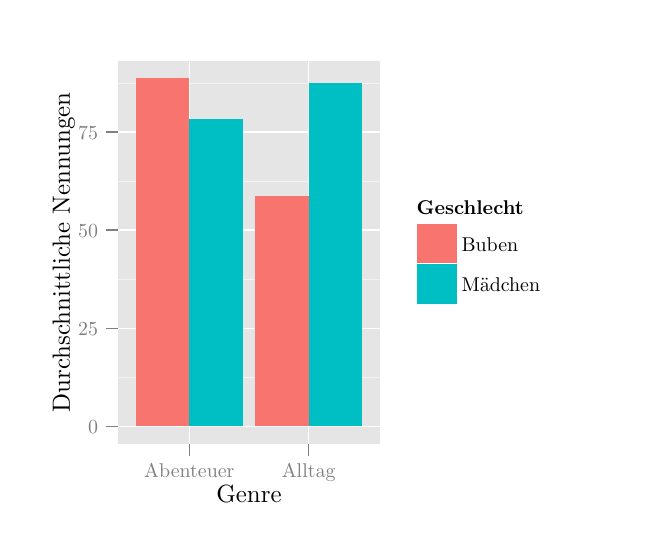
\begin{tikzpicture}[x=1pt,y=1pt]
\definecolor[named]{fillColor}{rgb}{1.00,1.00,1.00}
\path[use as bounding box,fill=fillColor,fill opacity=0.00] (0,0) rectangle (216.81,180.67);
\begin{scope}
\path[clip] (  0.00,  0.00) rectangle (216.81,180.67);
\definecolor[named]{drawColor}{rgb}{1.00,1.00,1.00}
\definecolor[named]{fillColor}{rgb}{1.00,1.00,1.00}

\path[draw=drawColor,line width= 0.6pt,line join=round,line cap=round,fill=fillColor] (  0.00,  0.00) rectangle (216.81,180.67);
\end{scope}
\begin{scope}
\path[clip] ( 32.55, 30.32) rectangle (127.38,168.63);
\definecolor[named]{fillColor}{rgb}{0.90,0.90,0.90}

\path[fill=fillColor] ( 32.55, 30.32) rectangle (127.38,168.63);
\definecolor[named]{drawColor}{rgb}{0.95,0.95,0.95}

\path[draw=drawColor,line width= 0.3pt,line join=round] ( 32.55, 54.31) --
	(127.38, 54.31);

\path[draw=drawColor,line width= 0.3pt,line join=round] ( 32.55, 89.73) --
	(127.38, 89.73);

\path[draw=drawColor,line width= 0.3pt,line join=round] ( 32.55,125.15) --
	(127.38,125.15);

\path[draw=drawColor,line width= 0.3pt,line join=round] ( 32.55,160.57) --
	(127.38,160.57);
\definecolor[named]{drawColor}{rgb}{1.00,1.00,1.00}

\path[draw=drawColor,line width= 0.6pt,line join=round] ( 32.55, 36.60) --
	(127.38, 36.60);

\path[draw=drawColor,line width= 0.6pt,line join=round] ( 32.55, 72.02) --
	(127.38, 72.02);

\path[draw=drawColor,line width= 0.6pt,line join=round] ( 32.55,107.44) --
	(127.38,107.44);

\path[draw=drawColor,line width= 0.6pt,line join=round] ( 32.55,142.86) --
	(127.38,142.86);

\path[draw=drawColor,line width= 0.6pt,line join=round] ( 58.42, 30.32) --
	( 58.42,168.63);

\path[draw=drawColor,line width= 0.6pt,line join=round] (101.52, 30.32) --
	(101.52,168.63);
\definecolor[named]{fillColor}{rgb}{0.97,0.46,0.43}

\path[fill=fillColor] ( 39.02, 36.60) rectangle ( 58.42,162.34);
\definecolor[named]{fillColor}{rgb}{0.00,0.75,0.77}

\path[fill=fillColor] ( 58.42, 36.60) rectangle ( 77.81,147.70);
\definecolor[named]{fillColor}{rgb}{0.97,0.46,0.43}

\path[fill=fillColor] ( 82.12, 36.60) rectangle (101.52,119.68);
\definecolor[named]{fillColor}{rgb}{0.00,0.75,0.77}

\path[fill=fillColor] (101.52, 36.60) rectangle (120.92,160.77);
\end{scope}
\begin{scope}
\path[clip] (  0.00,  0.00) rectangle (216.81,180.67);
\definecolor[named]{drawColor}{rgb}{0.50,0.50,0.50}

\node[text=drawColor,anchor=base east,inner sep=0pt, outer sep=0pt, scale=  0.72] at ( 25.44, 34.12) {0};

\node[text=drawColor,anchor=base east,inner sep=0pt, outer sep=0pt, scale=  0.72] at ( 25.44, 69.54) {25};

\node[text=drawColor,anchor=base east,inner sep=0pt, outer sep=0pt, scale=  0.72] at ( 25.44,104.96) {50};

\node[text=drawColor,anchor=base east,inner sep=0pt, outer sep=0pt, scale=  0.72] at ( 25.44,140.38) {75};
\end{scope}
\begin{scope}
\path[clip] (  0.00,  0.00) rectangle (216.81,180.67);
\definecolor[named]{drawColor}{rgb}{0.50,0.50,0.50}

\path[draw=drawColor,line width= 0.6pt,line join=round] ( 28.29, 36.60) --
	( 32.55, 36.60);

\path[draw=drawColor,line width= 0.6pt,line join=round] ( 28.29, 72.02) --
	( 32.55, 72.02);

\path[draw=drawColor,line width= 0.6pt,line join=round] ( 28.29,107.44) --
	( 32.55,107.44);

\path[draw=drawColor,line width= 0.6pt,line join=round] ( 28.29,142.86) --
	( 32.55,142.86);
\end{scope}
\begin{scope}
\path[clip] (  0.00,  0.00) rectangle (216.81,180.67);
\definecolor[named]{drawColor}{rgb}{0.50,0.50,0.50}

\path[draw=drawColor,line width= 0.6pt,line join=round] ( 58.42, 26.05) --
	( 58.42, 30.32);

\path[draw=drawColor,line width= 0.6pt,line join=round] (101.52, 26.05) --
	(101.52, 30.32);
\end{scope}
\begin{scope}
\path[clip] (  0.00,  0.00) rectangle (216.81,180.67);
\definecolor[named]{drawColor}{rgb}{0.50,0.50,0.50}

\node[text=drawColor,anchor=base,inner sep=0pt, outer sep=0pt, scale=  0.72] at ( 58.42, 18.24) {Abenteuer};

\node[text=drawColor,anchor=base,inner sep=0pt, outer sep=0pt, scale=  0.72] at (101.52, 18.24) {Alltag};
\end{scope}
\begin{scope}
\path[clip] (  0.00,  0.00) rectangle (216.81,180.67);
\definecolor[named]{drawColor}{rgb}{0.00,0.00,0.00}

\node[text=drawColor,anchor=base,inner sep=0pt, outer sep=0pt, scale=  0.90] at ( 79.97,  9.03) {Genre};
\end{scope}
\begin{scope}
\path[clip] (  0.00,  0.00) rectangle (216.81,180.67);
\definecolor[named]{drawColor}{rgb}{0.00,0.00,0.00}

\node[text=drawColor,rotate= 90.00,anchor=base,inner sep=0pt, outer sep=0pt, scale=  0.90] at ( 15.23, 99.47) {Durchschnittliche Nennungen};
\end{scope}
\begin{scope}
\path[clip] (  0.00,  0.00) rectangle (216.81,180.67);
\definecolor[named]{fillColor}{rgb}{1.00,1.00,1.00}

\path[fill=fillColor] (136.25, 76.46) rectangle (195.90,122.49);
\end{scope}
\begin{scope}
\path[clip] (  0.00,  0.00) rectangle (216.81,180.67);
\definecolor[named]{drawColor}{rgb}{0.00,0.00,0.00}

\node[text=drawColor,anchor=base west,inner sep=0pt, outer sep=0pt, scale=  0.72] at (140.52,113.25) {\bfseries Geschlecht};
\end{scope}
\begin{scope}
\path[clip] (  0.00,  0.00) rectangle (216.81,180.67);
\definecolor[named]{drawColor}{rgb}{1.00,1.00,1.00}
\definecolor[named]{fillColor}{rgb}{0.95,0.95,0.95}

\path[draw=drawColor,line width= 0.6pt,line join=round,line cap=round,fill=fillColor] (140.52, 95.18) rectangle (154.97,109.64);
\end{scope}
\begin{scope}
\path[clip] (  0.00,  0.00) rectangle (216.81,180.67);
\definecolor[named]{fillColor}{rgb}{0.97,0.46,0.43}

\path[fill=fillColor] (140.52, 95.18) rectangle (154.97,109.64);

\path[] (140.52, 95.18) --
	(154.97,109.64);
\end{scope}
\begin{scope}
\path[clip] (  0.00,  0.00) rectangle (216.81,180.67);
\definecolor[named]{drawColor}{rgb}{1.00,1.00,1.00}
\definecolor[named]{fillColor}{rgb}{0.95,0.95,0.95}

\path[draw=drawColor,line width= 0.6pt,line join=round,line cap=round,fill=fillColor] (140.52, 80.73) rectangle (154.97, 95.18);
\end{scope}
\begin{scope}
\path[clip] (  0.00,  0.00) rectangle (216.81,180.67);
\definecolor[named]{fillColor}{rgb}{0.00,0.75,0.77}

\path[fill=fillColor] (140.52, 80.73) rectangle (154.97, 95.18);

\path[] (140.52, 80.73) --
	(154.97, 95.18);
\end{scope}
\begin{scope}
\path[clip] (  0.00,  0.00) rectangle (216.81,180.67);
\definecolor[named]{drawColor}{rgb}{0.00,0.00,0.00}

\node[text=drawColor,anchor=base west,inner sep=0pt, outer sep=0pt, scale=  0.72] at (156.78, 99.93) {Buben};
\end{scope}
\begin{scope}
\path[clip] (  0.00,  0.00) rectangle (216.81,180.67);
\definecolor[named]{drawColor}{rgb}{0.00,0.00,0.00}

\node[text=drawColor,anchor=base west,inner sep=0pt, outer sep=0pt, scale=  0.72] at (156.78, 85.48) {Mädchen};
\end{scope}
\end{tikzpicture}

  \caption[Unterschiede zwischen Abenteuer und Alltag]{Unterschiede zwischen Abenteuer und Alltag bei Mädchen und Buben}
\end{figure}

Alltagsgeschichten spielen in einem dem Hauptprotagonisten vertrauten
Umfeld. Bei kindlichen Protagonisten handelt es sich zumeist um die
familiäre und/oder schulische Umgebung. Es werden Themen und
Problematiken angesprochen, die im realen Leben der Leser und Leserinnen
mit großer Wahrscheinlichkeit vorkommen können. Beispiele dafür sind
Beziehungsprobleme mit Freunden, Eltern oder Lehrern, aber auch
Leistungsdruck in der Schule, Erlebnisse auf Klassenfahrten, Urlaube
oder der Tod von Haustieren. Wir konnten feststellen, dass
Alltagsgeschichten deutlich häufiger von Mädchen gelesen werden.

\subsubsection{Beispiel: Alltagsgeschichte}

``Das ist Lilli, die Hauptperson unserer Geschichte. Sie ist ungefähr so
alt wie du und sieht aus wie ein gewöhnliches Kind.''
\parencite[][6]{KNISTER1999} Bereits der erste Satz des Buches Hexe
Lilli zeigt, wie nahe der Charakter am ``realen'' Leben angelegt ist.
Kinder sollen sich von Anfang an mit dem Hauptcharakter identifiziern.
Lilli durchlebt in den Büchern ihren Alltag gespickt mit Erlebnissen die
keinem der jungen Leser und keiner Leserin zur Gänze unbekannt sind.
Spielen mit dem kleinen Bruder, sowie Unverständnis über die
Einstellungen der Eltern gehören wohl zu jedem vielfältigen
Kinderalltag.

Die kleine Hexe Lilli ist nicht nur ein Beispiel einer
Alltagsgeschichte. Zusätzlich kann sie als Beispiel einer Protagonistin
mit ausgeglichenem Genderwert genannt werden. Lilli vereinigt in sehr
ausgeglichener Weise sowohl maskuline als auch feminine Eigenschaften.
So ist sie etwa auch dominant und tatkräftig wie folgende Situation
zeigt:

Situationsbeschreibung: Der Schulrat besucht an diesem Tag die Klasse
von Lilli und möchte den Unterricht von Frau Grach, der Klassenlehrerin,
inspizieren. Lilli möchte der Frau Lehrerin gerne helfen einen guten
Eindruck zu hinterlasssen, doch der Herr Schulrat taucht natürlich genau
im falschen Moment auf als das totale Chaos in der Klasse herrscht.

\begin{quote}
``Auweia'', flüstert Lilli. So war das nicht gedacht! Hier muss sie
schnell eingreifen bevor der Schulrat gleich zu Anfang einen schlechten
Eindruck bekommt. \parencite[][47
]{KNISTER1999}
\end{quote}

Lilli bietet aus Sicht des Doing-Gender einen Mix an Eigenschaften, der
sich auch in ihrem Genderwert widerspiegelt. Lilli wird sehr klar
bevorzugt von Mädchen gelesen und zeigt, wie Mädchen ebenfalls mit
maskulinen Genderattributen dargestellt werden.

Beispiele für Alltagsgeschichten, die von Buben gelesen werden, sind
etwa \emph{Gregs Tagebuch} und \emph{Die wilden Fußballkerle}, doch auch
wenn diese zwei absolute Lieblingsbücher für Jungen zu sein scheinen,
stellen sie doch die Ausnahme dar.

\subsection{Abenteuergeschichten}

Abenteuergeschichten sind das Gegenstück zu Alltagsgeschichten. Dabei
durchlebt der Hauptprotagonist ein wahrscheinlich einzigartiges
Erlebnis, das zumeist mit großen Risiken und Gefahren verbunden ist. Der
Protagonist ist dabei zumeist gezwungen sein gewohntes Umfeld zu
verlassen und sich in völlig fremden oft auch unrealistischen
Situationen zurechtzufinden. Beispiele hierfür wären die Suche nach
einem verschollenen Schatz, das Tätigen einer gefährlichen und
ungewissen Reise, das Kämpfen mit bösen Mächten wie Ganoven, Drachen und
anderem. Wir konnten feststellen, dass Buben vor allem
Abenteuergeschichten favorisieren.

\subsubsection{Beispiel: Abenteuerbuch}

Harry ist ein schmächtiger Junge, der bei der Familie seiner Tante lebt,
da seine Eltern gestorben sind. Allerdings nur so lange bis er erfährt,
dass er ein Zauberer ist und auf die Zauberschule kommt. Dort angekommen
erlebt er ein Abenteuer nach dem anderen. Diese gipfeln in einem großen
und brutalen Show-Down im Kampf gegen den Mörder seiner Eltern.
\parencite{Rowling1998}

Harry Potter ist ein passendes Beispiel dafür, dass Jungen männliche und
maskuline Protagonisten, vor allem aber auch Abenteuergeschichten
favorisieren.

\subsection{Zusammenhänge inhaltlicher Merkmale}

Aus unserer Erhebung zur Darstellung von Gendermerkmalen wissen wir,
dass gewisse Eigenschaften als besonders maskulin oder feminin empfunden
werden. Wir haben uns daher gefragt, ob es denn Merkmale im Inhalt und
Aufbau von Kinderbüchern geben könnte, die die Ausprägung solcher
Eigenschaften unterstützen. Da die Ergebnisse für Jungen viel
einseitiger ausgefallen sind, kann die Frage auch wie folgt formuliert
werden: Weisen Abenteuergeschichten bestimmte Merkmale auf mit denen
Buben verstärkt konfrontiert werden, die zur Entwicklung
\emph{maskuliner} Eigenschaften beitragen könnten? Oder: Fehlen durch
das sparsame Lesen von Alltagsgeschichten bestimmte Merkmale, die eine
femininere Entwicklung verhindern?

Folgende vier Kriterien wurden erhoben, bei denen von einem Einfluss auf
die Geschlechterrollenentwicklung ausgegangen wurde:

\subsubsection{Quest}

Verläuft die Geschichte des Buches auf ein bestimmtes Ziel hin, das
erreicht werden soll? Erfordert das Erreichen des Zieles das Lösen von
Aufgaben bzw. Rätseln? Besonders Kriminal- und Detektivgeschichten sind
mit einem obersten Ziel verknüpft, dass erreicht werden soll. Auf dem
Weg bis zur Lösung stellen sich dem Protagonisten Stolpersteine in den
Weg, die zuerst entfernt werden müssen. Dies braucht oft rationales
Denken, Mut, aktives Handeln oftmals auch körperliche Stärke und
Aggression. All diese Attribute werden im Sinne des Doing-Gender als
maskuline Eigenschaften wahrgenommen und könnten daher eine spezifische
Geschlechterrollenentwicklung miterklären. Es ist daher wenig
überraschend, dass die Präsenz von Quests in enger Verbindung mit
Abenteuergeschichten steht ($r= -0{,}548^{**}$). Der negative
Zusammenhang entsteht aufgrund der gegengleichen Polung der Variablen
(Alltag 1, Abenteuer 2; Quest vorhanden 1, nicht vorhanden 2).

\paragraph{Beispiel Quest:}

Die Knickerbockerbande besteht aus Lilo, Axel, Dominik und Poppi, die in
jedem Band neue \emph{Rätsel} lösen. Dabei kann es vorkommen, dass sie
etwa im Urlaub auf mysteriöse Fälle stoßen, die sie zu viert aufklären.
Das Quartett gerät öfter in Gefahr oder in die Hände von Verbrechern,
aus denen es sich aber mit List und Geschick wieder befreit. Dies ist
ein eindeutiger Indikator für das Merkmal des Quests. Die Hauptfiguren
haben unterschiedliche Qualitäten, können aber als ein Multiprotagonist
verstanden werden. Auch das Verhalten untereinander ist sehr
hilfsbereit, sie sind verlässlich und sie alle vereint dasselbe Hobby,
nennen wir es ``Dedektiv spielen'', worauf sie sich auch in ihrer
Freizeit vorbereiten und trainieren (etwa wie man sich anschleicht oder
besonders schnell ist). Die Geschichten wirken anfangs mysteriös, was
auch die Titel wiedergeben, die manchmal gruselige und surreale
Situationen zu versprechen scheinen, die sich dann aber immer als
menschengemacht herausstellen.

\begin{quote}
Die Männer in den roten Mänteln lagen kraftlos am Boden. \textelp{} Axel
waren sofort die kleinen roten Federbüschel aufgefallen, die ihnen
seitlich aus dem Hals ragten. Sie dienten einer kleinen Nadel als
Stabilisator. Solche Nadeln wurden aus Blasrohren abgefeuert. Axel
erinnerte sich, etwas im Fernsehen darüber gesehen zu haben.
\parencite[][117]{Brezina2010}
\end{quote}

Die Protagonisten agieren sehr rational. Sie können Situationen gut
einschätzen und verknüpfen das Wissen aus anderen Informationsquellen
mit dem Erlebten. Diese Eigenschaft hilft ihnen dabei die Rätsel zu
lösen und ihr Ziel zu erreichen.

\subsubsection{Phantastische Elemente}

Kommen in den Büchern Figuren, Orte oder Handlungen vor, die in der
Realität nicht vorkommen? Beispiele: Einhörner, sprechende Tiere,
fliegende Menschen, Zauberer, fremde Welten, uvm. Phantastische Elemente
könnten eine Tendenz zum träumerischen, irrationalen Denken fördern,
welches aus der Sicht des Doing-Genders feminine Attribute wären. Doch
Abenteuergeschichten sind natürlich gespickt mit unmöglichen
Situationen. Oftmals bekämpfen Charaktere Monster und Gespenster. Daher
tendieren die Zahlen dazu, das Vorkommen von phantastischen Elementen
den Abenteuerbüchern zuzuschreiben. Das niedrige Signifikanzniveau lässt
hier jedoch keine genaue Aussage zu. Es kann auch kein Zusammenhang mit
dem w/m-Faktor gefunden werden. Dieses inhaltliche Merkmal scheint in
beiden Geschlechtsgruppen annähernd gleich oft verwendet zu werden und
kann daher keine Annäherung zur Erklärung von Geschlechtsrollenbildung
liefern.

\subsubsection{Growing-Up:}

Verändert sich im Verlauf der Geschichte die Persönlichkeit des
Hauptprotagonisten? Durchläuft er einen Reifeprozess? Erhebt das Buch
den Anspruch eine pädagogische Nachricht zu vermitteln, hingerichtet auf
eine positive Sozialisierung? Mädchen gelten oftmals im Vergleich zu den
gleichaltrigen Jungen als sozial weiter entwickelt. Dieser Vorsprung in
der Entwicklung könnte zum Teil durch eine vermehrte Konfrontation mit
pädagogisch motivierter Literatur mitbegründet sein. Tatsächlich besteht
hier ein Zusammenhang mit dem Geschlecht der Lesenden
($r= 0{,}384; p= 0{,}07$), wenn wir über das leicht erhöhte
Signivikanzniveau hinwegsehen. Unter denselben Umständen kann auch eine
positive Korrelation mit dem Merkmal des Inneren Monologs festgestellt
werden ($r= 0{,}399; p= 0{,}066$), sowie eine signifikante negative
Korrelation mit dem Merkmal Quest ($r= -0{,}466^*$). Das bedeutet, dass
Kombinationen dieses Merkmals mit dem Merkmal ``Innerer Monolog''
oftmals vorkommen, wärend Reifeprozesse und Quests eher selten im selben
Buch zu finden sind.

Ein geradezu idealtypisches Beispiel für ein Buch, das einen
Reifeprozess thematisiert, stellt etwa die Geschichte des Pinocchio dar,
der auf seinem Weg ein richtiger Junge zu werden, vor allem lernen muss,
wie sich ein Mensch zu benehmen hat. So wird etwa das Lügen nicht
geduldet und führt zu Konsequenzen.

\subsubsection{Innerer Monolog}

Welche Rolle spielt die Gedankenwelt des Hauptprotagonisten? Wie stark
reflektiert er seine Entscheidungen vor und/oder nach dem Handeln? Wie
intensiv wird sie dem Leser/der Leserin vermittelt? Mädchen gelten als
passiver und introvertierter als ihre männlichen Altersgenossen und
haben aus Sicht des Doing-Gender ein größeres Einfühlungsvermögen als
Jungen. All dies wären Indizien den Inneren Monolog als ein Merkmal zu
deklarieren, das Jungen fehlen könnte, um eine feminine Seite zu
entwickeln. Und tatsächlich tendieren die Zahlen unserer Ergebnisse
dazu, einen Zusammenhang von Alltagsgeschichten und Innerem Monolog zu
bescheinigen. Auch hier ist jedoch das Signifikanzniveau zu niedrig um
fixe Aussagen zu tätigen. Interpretieren wir zusätzlich Ergebnisse deren
Signivikanzniveaus leicht über $0{,}05$ liegen, fällt auf, dass das
Merkmal Innerer Monolog negativ mit dem Merkmal Quests korreliert
($r= -0{,}376; p= 0{,}084$). Das bedeutet, dass das kombinierte
Vorkommen dieser beiden Merkmale äußerst selten anzutreffen ist.
Zusätzlich besteht unter den selben Umständen ein Zusammenhang mit dem
Vorkommen von Reifeprozessen ($r= 0{,}399; p= 0{,}066$). Dies lässt die
Aussage zu, dass diese Kombination scheinbar von AutorInnen gerne
gewählt wird.

\paragraph{Beispiel Innerer Monolog:}

In den Mini-Büchern geht es darum, den frühen Alltag eines Kindes zu
bewältigen und persönliche Konflikte auf sehr humorvolle Art aus Minis
Sicht wiederzugeben.

Mini ist schon sehr groß für ihr Alter und gleichzeitig sehr dünn,
weshalb ihr auch alle möglichen Spitznamen gegeben werden, was sie
kränkt. Der Schule blickt sie mit gemischten Gefühlen entgegen,
gleichzeitig freut sie sich schon drauf, hat aber auch Angst in die
falsche Schule zu kommen, von der falschen Lehrerin unterrichtet zu
werden oder vor den fremden Kindern, die sie wieder hänseln könnten.
Dies zeigt wie viel sie reflektiert und über mögliche Situationen und
Folgen nachdenkt. Als Beispiel kann hier der Gedankengang genannt
werden, der zeigt wie erleichtert sie darüber ist, dass sie nicht die
Größte in ihrer Klasse ist:

\begin{quote}
Und die Mini fing vor lauter Staunen zu schielen an. \textelp{} Warum
die Mini so erstaunt und verblüfft war? Weil sie garantiert nicht das
größte Kind ihrer Klasse war! Ein Bub und ein Mädchen waren noch ein
bisschen größer als die Mini, 2 Buben und 2 Mädchen waren genauso groß
wie die Mini. Die Mini dachte:``Wenn es unter zwanzig Kindern sieben
lange Latten gibt, dann ist ja die Überlänge direkt normal!''
\parencite[][61]{Noestlinger2011}
\end{quote}

Die Untersuchung der vier inhaltlichen Merkmale von Alltags- und
Abenteuergeschichten konnte vor allem zeigen, dass eine Analyse anhand
von 23 Büchern keine wirklich aussagekräftigen Ergebnisse liefern kann
und hier eine große eigenständige Untersuchung notwendig wäre um etwaige
Zusammenhänge zwischen inhaltlichen Merkmalen und der Ausprägungen von
geschlechterspezifischen Eigenschaftsmerkmalen genau zu untersuchen.
Somit bleibt hier als einzig aussagekräftiges Ergebnis nur die
Erkenntnis, dass sich die Buben vor allem auf Abenteuergeschichten
konzentrieren, Alltagsgeschichten hingegen vermehrt von Mädchen gelsen
werden. Einzelne Merkmale konnten zwar auf ihr vermehrtes Aufkommen in
Alltags- und Abenteuergeschichten untersucht werden und Tendenzen
erkannt werden. Um jedoch aussagekräftige Rückschlüsse auf ihren
Einfluss und ihre Konzentration bei den Geschlechtern ziehen zu können,
sind weitere Untersuchungen notwendig. Diese Arbeit konnte lediglich
aufzeigen, dass dies durchaus interessante Ergebnisse liefern könnte.

\section{Sonderkapitel: Fünf Freunde}

Hier soll in ein paar wenigen Zeilen erklärt werden, warum wir bei den
Fünf Freunden nicht fähig waren, trotz aller Bemühungen, einen
Hauptprotagonisten zu finden und die spannende Buchreihe somit bei den
Analysen der Darstellung des Genders nicht berücksichtigt werden konnte.
Dieses kleine Spezialkapitel soll den Verlust des meistgenannten Buches
bei der Analyse der Genderdarstellungen zumindest etwas ausgleichen und
die Charaktäre trotzdem vorstellen, auch wenn der w/m-Faktor (siehe:
Tabelle 3.1.) nur einen sehr ausgeglichenen Wert für dieses Buch hergibt
und somit nur schwer einem Geschlecht zugeordnet werden kann. Um so
interessanter ist, dass beide Geschlechter die Geschichten der Fünf
Freunde noch immer verfolgen. Neben der Tatsache, dass es sich bei den
Fünf Freunden um eine Abenteuergeschichte handelt, die sowohl von Buben
als auch von Mädchen gelesen wird, lohnt es sich, sich die
Genderausprägungen der vier Protagonisten anzusehen. Die Fünf Freunde
bestehen aus zwei weiblichen und zwei männlichen Protagonisten, die von
ihrem vierbeinigen Freund Timmy begleitet werden. Da alle vier eine
annähernd gleich starke Bedeutung im Geschichtsverlauf haben, war die
Selektion auf einen einzelnen Charakter schlichtweg nicht möglich. Somit
wurde die Gruppe hingehend auf die Bildung eines Multiprotagonisten
untersucht. Das gemeinsame Ziel und Vorgehen hätte auch stark für die
Bildung eines solchen gesprochen. Jedoch war die generelle Darstellung
des Genders der ProtagonistInnen ein Problem für die Bildung eines
Multiprotagonsten. Während die Verhaltens- und Handlungsweisen der
beiden Jungen (Julius und Richard) ihrem Geschlecht zuordbar sind, da
beide vor allem aber Julius als Ältester und Anführer doch sehr maskulin
agieren. Das Scheitern eines Multiprotagonisten liegt vielmehr in der
Darstellung der weiblichen Charaktere begründet. Während Georgina sehr
maskulin dargestellt wird und auch ein Junge sein möchte - sie möchte
Georg genannt werden - und somit sehr gut mit den Genderwerten der
Jungen kombinierbar wäre, gibt es mit Anne ein Problem. Diese wird
nämlich so feminin dargestellt, dass ein Mittelwert aller vier
menschlichen Charaktere sich als relativ geschlechtsneutral zeigen
würde. Da dies jedoch nicht die Darstellungen im Buch widergespiegelt
hätte, wurde die Buchreihe bei der Untersuchung nicht berücksichtigt.

Die unterschiedliche Darstellung der beiden Mädchen wird bei folgender
Textstelle sichtbar, bei der die Fünf Freunde sich auf Spurensuche
befinden:

\begin{quote}
``Wir werden uns furchtbar schmutzig machen und nachher aussehen wie die
Schornsteinfeger'', gab Anne zu bedenken. ``Schmutzig werden! Du hast
wohl einen Sprung in der Schüssel!'' rief Georg{[}ina{]} empört. ``Wer
kümmert sich denn darum, bei so einer wichtigen
Entdeckung!''\parencite[][138]{Blyton2009}
\end{quote}

Wagen wir uns hier einen Grund zu finden warum beide Geschlechter die
Bücherreihe von Enid Blyton lesen, so könnte davon ausgegangen werde,
dass die Jungen vor allem von den Abenteuergeschichten und der Überzahl
an maskulinen Charakteren (Julius, Richard, Georgina) angezogen werden.
Unsere Ergebnisse sagen uns, dass auch Mädchen von Abenteuergeschichten
nicht abgeneigt sind und über Charaktere beider Genderausprägungen
lesen. Sie bevorzugen zwar weibliche Protagonisten, diese können jedoch
sowohl maskulin als auch feminin dargestellt werden. Beides finden wir
bei den Fünf Freunden. Auf der einen Seite die starke und
durchsetzungsfähige Georg und auf der anderen die mädchenhafte Anne. Die
beiden Protagonistinnen verkörpern die Extrempole und reiben sich an
diesen. Zum Vergleich: Auch bei der Knickerbockerbande gibt es zwei
Mädchen, die aber beide männliche und weibliche Eigenschaften vereinen
und keine Antagonisten sind. Somit kann resümiert werden, dass auch die
Fünf Freunde und ihre Beliebtheit bei beiden Geschlechtern anhand
unserer Herangehensweise und Ergebnisse erklärt werden können.

\section{Fazit und Verknüpfung mit der Theorie}

Wir konnten mit unseren Erbenissen das Wissen, dass Mädchen Bücher mit
weiblichen und Buben welche mit männlichen Charakteren lesen und den
damit von uns verbundenen Annahmen (H 2, H 2.1, H 2.2) bestätigen. Als
großer Triumpf dieses Kapitels ist die Untersuchung der Gendermerkmale
von Hauptprotagonisten in Kinderbüchern zu sehen. Sie hat uns gezeigt,
dass Buben vor allem über maskuline Charaktere lesen, Mädchen hingegen
mit beiden konfrontiert werden (H 3, H 3.1, H 3.2). Nachwievor scheinen
manche stereotype Eigenschaften bestimmten Geschlechtern zugeschrieben
zu werden, womit der Prozess des Gender-Mainstreaming behindert werden
könnte. Das Gender kann hier ergänzend zum Geschlecht gesehen werden um
das Doing-Gender von Kinderbuchcharakteren zu erklären. Die Erhebung
über inhaltliche Merkmale führte zu interessanten Erkenntnissen über
Alltags- und Abenteuergeschichten und ihr Zusammenhang mit dem
Geschlechtsverhältnis der Lesenden (H 4.1). Denn obwohl Abenteuerbücher
von beiden Geschlechtern gelesen werden, werden Alltagsgeschichten
eindeutig verstärkt Mädchen konsumiert. Bei den inhaltlichen Merkmalen
sind jedoch noch weitere Untersuchungen notwendig, da die Arbeit
lediglich Anhaltspunkte und Zuversicht bezüglich möglicher
aussagekräftiger Ergebnisse liefern konnte. So konnten zwar die Annahmen
zur Kathegorie Quest bestätigt werden (H 4.2), während die Merkmale
Innerer Monolog und Growing Up lediglich Tendenzen wiedergeben konnten
(H 4.3, H 4.4). Die Annahme das phantastische Elemente besonders in den
von Mädchen favorisierten Büchern zu finden sind, konnte nicht bestätigt
werden (H 4.5). Der Versuch dieses Ergebnis mit Theorie zu verknüpfen
kann zu provokanten Aussagen führen, die hier nur genannt werden um
etwaige Untersuchungen in der Zukunft zu motivieren. So kann etwa unser
Wissen, dass Mädchen und Buben unterschiedliche Bücher lesen mit der
Theorie verknüpft werden, dass das Verhalten von Protagonisten in
Büchern auf deren Leser abfärbt und somit Verhalten reproduziert. Diese
Verknüpfung würde aus Sicht der Ergebnisse dieser Untersuchung wie folgt
zu interpretieren sein: Wenn Buben verstärkt mit maskulinen
Protagonisten konfrontiert werden, könnte diese Einseitigkeit zu einer
Stabilisierung von stereotypen Geschlechterrollen führen. Bei Mädchen
hingegen sagen uns die Ergebnisse, dass sie inzwischen mit
vielfältigeren Eigenschaften und Handlungsalternativen konfrontiert
werden und daher im Sinne des Gender-Mainstreamings eine größere Chance
haben, bestehende stereotype Rollenbilder zu brechen und neu zu
gestalten.

\chapter{Äußere Merkmale, die das Leseverhalten erklären}

In \thref{h5} (siehe Seite \pageref{h5}) nehmen wir an, dass das
Verhältnis von Leserinnen zu Lesern (\emph{w/m-Faktor}), allein durch
\emph{oberflächliche} Merkmale zu erklären ist. Obeflächliche Merkmale
des Buchs sind vor allem Merkmale des Umschlags, wie Hellgikeit,
Geschlecht der Titelfigur oder ob es sich um eine Autorin oder einen
Autor
handelt.\footnote{Die Merkmale werden auf Seite \pageref{meth.merkmale} genau beschrieben.}
Um die Hypothese zu überprüfen, stellen wir ein lineares Modell mit den
in Frage kommenden Merkmalen auf und testen so, wie gut sie das
Geschlechterverhältnis der Lesenden erklären können. Danach schauen wir
uns die einzelnen Merkmale und ausgewählten Merkmalskombinationen an.

Das beste
Modell\footnote{Unter \enquote{bestem Modell} verstehen wir das Modell mit dem höchsten korrigierten Bestimmtheitsmaß (\(R_{kor.}\))}
(Modell 1 in Tabelle \ref{wmmodel}) setzt sich aus drei Merkmalen eines
Kinderbuchs zusammen: dem \emph{Geschlecht der Titelfigur}, der
\emph{Helligkeit} und der \emph{Anzahl der Seiten}. Diese reichen aus,
um das Verhältnis von Leserinnen zu Lesern bei einem Kinderbuch
voraussagen zu können. Das Modell kann mit einer Genauigkeit von rund
80\% ($R_{kor.}0{,}82$) das Geschlechterverhältnis voraussagen. Wobei
das Vorhandensein eines weiblichen Namens im Titel mit Abstand am
meisten zu dem Modell beiträgt ($\beta=-0{,}77$). Wenn ein weiblicher
Name im Titel vorkommt, lesen das Buch viel mehr Mädchen als Buben. Mit
einigem Abstand in der Wichtigkeit, aber noch immer deutlich
ausschlaggebend, kommt die Helligkeit des Covers ($\beta=0{,}29$). Je
heller ein Buch ist, umso größer ist der Anteil der Mädchen, die das
Buch lesen. Die Anzahl der Seiten dient dann nur noch zur Verfeinerung
($\beta=0{,}19$). Hier fiel das Ergebnis, auf den ersten Blick, für uns
überraschend aus, denn je dicker ein Buch ist, umso höher ist der Anteil
der Buben, die das Buch lesen. All diese Merkmale können von Kindern
ohne Probleme und ohne, dass sie das Buch aufmachen müssen wahrgenommen
werden. Die \thref{h5} können wir somit auch \thref{fra:merkmale}
eindeutig mit \emph{ja} beantworten. Steht im Titel ein weiblicher Name,
ist das Buch noch dazu sehr hell und obendrein auch noch dünn. Dann ist
die Wahrscheinlichkeit sehr hoch, dass das Buch viel mehr Mädchen als
Buben gelesen haben. Ist das Buch dunkel, dick und kommt kein weiblicher
Name im Titel vor, ist es wahrscheinlicher, dass der Anteil der Leser
höher ist.

      
      \ctable[
      %  cap    = ,
        caption = {Lineare Modelle die den w/m-Faktor erklären},
        label   = wmmodel ,
        pos   = htp,
      %  width    = \textwidth
      ]{lD{,}{,}{2}D{,}{,}{2}D{,}{,}{2}}{
        % \tnote[.]{< 0,1}
        % \tnote[*]{< 0,05}
        % \tnote[**]{< 0,01}
        % \tnote[***]{< 0,001}
      }{                  
      \FL 
      \small   &  
      \multicolumn{1}{c}{\small Modell 1} & 
      \multicolumn{1}{c}{\small Modell 2} & 
      \multicolumn{1}{c}{\small Modell 3}
      \ML Geschlecht Titelfigur (unbestimmt)    & 0,06      & 0,02      &
      \NN Geschlecht Titelfigur (weiblich)      & -0,77\tmark[***]     & -0,82\tmark[***]     & 
      \NN Geschlecht Titelfigur (männlich)      & \multicolumn{1}{c}{ref.}      & \multicolumn{1}{c}{ref.}      & 
      \NN Coverhelligkeit                       & -0,29\tmark[**]     &           & -0,46\tmark[**]
      \NN Seitenanzahl                          & 0,19\tmark[*]      &           & 
      \ML Korrigiertes $R^2$                    & 0,82\tmark[***]      & 0,69\tmark[***]      & 0,18\tmark[**]  
      \LL \multicolumn{4}{l}{\footnotesize  $^*p<0{,}05, ^{**}p<0{,}01, ^{***}p<0{,}001$}
      }
      

      
      \ctable[
      %  cap    = ,
        caption = {Lineare Modelle die den w/m-Faktor erklären},
        label   = wmmodel ,
        star,
        pos   = htp,
      %  width    = \textwidth
      ]{lD{,}{,}{2}D{,}{,}{2}D{,}{,}{2}}{
        % \tnote[.]{< 0,1}
        % \tnote[*]{< 0,05}
        % \tnote[**]{< 0,01}
        % \tnote[***]{< 0,001}
      }{                  
      \FL 
      \small   &  
      \multicolumn{1}{c}{\small Modell 1} & 
      \multicolumn{1}{c}{\small Modell 2} & 
      \multicolumn{1}{c}{\small Modell 3}
      \NN 
      \small erklärte Variable  &  
      \multicolumn{1}{c}{\small \emph{w/m-Faktor}} & 
      \multicolumn{1}{c}{\small Mädchen} & 
      \multicolumn{1}{c}{\small Buben}
      \ML Geschlecht Titelfigur (unbestimmt)    & 0,06      & 0,02      &
      \NN Geschlecht Titelfigur (weiblich)      & -0,77\tmark[***]     & -0,82\tmark[***]     & 
      \NN Geschlecht Titelfigur (männlich)      & \multicolumn{1}{c}{ref.}      & \multicolumn{1}{c}{ref.}      & 
      \NN Coverhelligkeit                       & -0,29\tmark[**]     &           & -0,46\tmark[**]
      \NN Seitenanzahl                          & 0,19\tmark[*]      &           & 
      \ML Korrigiertes $R^2$                    & 0,82\tmark[***]      & 0,69\tmark[***]      & 0,18\tmark[**]  
      \LL \multicolumn{4}{l}{\footnotesize  $^*p<0{,}05, ^{**}p<0{,}01, ^{***}p<0{,}001$}
      }
      

      
      \ctable[
      %  cap    = ,
        caption = {Lineare Modelle ohne Vorlesebücher},
        label   = models26 ,
        star,
        % pos   = htp,
      %  width    = \textwidth
      ]{lD{,}{,}{2}D{,}{,}{2}D{,}{,}{2}}{
        % \tnote[.]{< 0,1}
        % \tnote[*]{< 0,05}
        % \tnote[**]{< 0,01}
        % \tnote[***]{< 0,001}
      }{                  
      \FL 
      \small   &  
      \multicolumn{1}{c}{\small Modell 7} & 
      \multicolumn{1}{c}{\small Modell 8} & 
      \multicolumn{1}{c}{\small Modell 9}
      \NN 
      \small erklärte Variable  &  
      \multicolumn{1}{c}{\small \emph{w/m-Faktor}} & 
      \multicolumn{1}{c}{\small Mädchen} & 
      \multicolumn{1}{c}{\small Buben}
      \ML Geschlecht Titelfigur (männlich)    & -0,05      & 0,11      & 0,16
      \NN Geschlecht Titelfigur (weiblich)    & -0,84\tmark[***] & 0,51\tmark[*] & -0,47\tmark[*]
      \NN Geschlecht Titelfigur (unbest.)     & \multicolumn{1}{c}{ref.} & \multicolumn{1}{c}{ref.} & \multicolumn{1}{c}{ref.}
      \NN Coverhelligkeit                     & -0,26\tmark[*]  & 0,02    & -0,29
      \NN Seitenanzahl                        & 0,06    & 0,14    & 0,14
      \NN Anzahl d. Figuren am Cover          & 0,07             & -0,42\tmark[*]   & -0,17
      \ML Korrigiertes $R^2$         & 0,82\tmark[***]  & 0,28      & 0,43\tmark[**]
      \LL \multicolumn{4}{l}{\footnotesize  $^*p<0{,}05, ^{**}p<0{,}01, ^{***}p<0{,}001$}
      }
      

\section{Unterschiede zwischen Mädchen und Buben}

Die Gefahr bei der Interpretation von Modellen, die den
\emph{w/m-Faktor} erklären, ist, dass man meinen könnte, die Faktoren
wirken automatisch auf die Anzahl der Mädchen und Buben, die ein Buch
gelesen haben. Der \emph{w/m-Faktor} ist das Verhältnis von Leserinnen
zu Lesern. Das heißt, auch Faktoren, die nur die Mädchen oder nur die
Buben beeinflussen, schlagen sich auf das Geschlechterverhältnis nieder.

Dafür, dass ein Buch von vielen Mädchen gelesen wird, ist es wichtig,
dass ein weiblicher Name im Titel vorkommt und dass möglichst wenig
Figuren am Cover sichtbar sind. (Siehe Modell 5 in Tabelle
\ref{models2}) Die Dicke eines Buchs ist für die Anzahl der Leserinnen
wenig ausschlaggebend und von der Helligkeit kann gar kein Einfluss
nachgewiesen werden.

Diese Merkmale sind für die Häufigkeit mit der Buben ein Buch lesen
natürlich umso wichtiger. Das für die Anzahl der Buben, die ein Buch
lesen, dieselben Faktoren, wie für den \emph{w/m-Faktor}, wichtig sind,
lässt darauf schließen, dass der \emph{w/m-Faktor} zu einem größeren
Teil vom Leseverhalten der Buben, als dem der Mädchen erklärt wird. Und
tatsächlich ist die Korrelation zwischen der Häufigkeit der Nennungen
pro Buch bei den Buben und dem Verhältnis der Nennungen zwischen Mädchen
und Buben mit $0{,}70$ größer als zwischen den Mädchen und dem
Verhältnis, dass nur eine Korrelation von $-0{,}41$ aufweist.

\section{Das Geschlecht der Titelfigur}

\begin{figure}
\center
  \label{titelfig}
  \small
% Created by tikzDevice version 0.6.2-92-0ad2792 on 2013-02-15 18:44:34
% !TEX encoding = UTF-8 Unicode
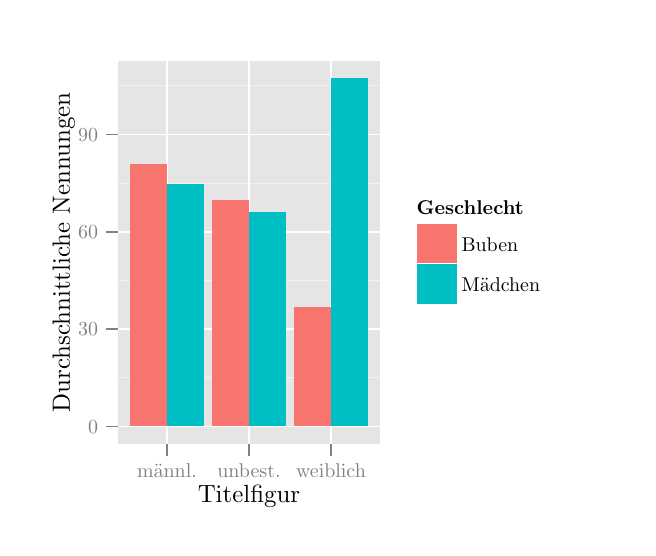
\begin{tikzpicture}[x=1pt,y=1pt]
\definecolor[named]{fillColor}{rgb}{1.00,1.00,1.00}
\path[use as bounding box,fill=fillColor,fill opacity=0.00] (0,0) rectangle (216.81,180.67);
\begin{scope}
\path[clip] (  0.00,  0.00) rectangle (216.81,180.67);
\definecolor[named]{drawColor}{rgb}{1.00,1.00,1.00}
\definecolor[named]{fillColor}{rgb}{1.00,1.00,1.00}

\path[draw=drawColor,line width= 0.6pt,line join=round,line cap=round,fill=fillColor] (  0.00,  0.00) rectangle (216.81,180.67);
\end{scope}
\begin{scope}
\path[clip] ( 32.55, 30.32) rectangle (127.38,168.63);
\definecolor[named]{fillColor}{rgb}{0.90,0.90,0.90}

\path[fill=fillColor] ( 32.55, 30.32) rectangle (127.38,168.63);
\definecolor[named]{drawColor}{rgb}{0.95,0.95,0.95}

\path[draw=drawColor,line width= 0.3pt,line join=round] ( 32.55, 54.18) --
	(127.38, 54.18);

\path[draw=drawColor,line width= 0.3pt,line join=round] ( 32.55, 89.34) --
	(127.38, 89.34);

\path[draw=drawColor,line width= 0.3pt,line join=round] ( 32.55,124.50) --
	(127.38,124.50);

\path[draw=drawColor,line width= 0.3pt,line join=round] ( 32.55,159.66) --
	(127.38,159.66);
\definecolor[named]{drawColor}{rgb}{1.00,1.00,1.00}

\path[draw=drawColor,line width= 0.6pt,line join=round] ( 32.55, 36.60) --
	(127.38, 36.60);

\path[draw=drawColor,line width= 0.6pt,line join=round] ( 32.55, 71.76) --
	(127.38, 71.76);

\path[draw=drawColor,line width= 0.6pt,line join=round] ( 32.55,106.92) --
	(127.38,106.92);

\path[draw=drawColor,line width= 0.6pt,line join=round] ( 32.55,142.08) --
	(127.38,142.08);

\path[draw=drawColor,line width= 0.6pt,line join=round] ( 50.33, 30.32) --
	( 50.33,168.63);

\path[draw=drawColor,line width= 0.6pt,line join=round] ( 79.97, 30.32) --
	( 79.97,168.63);

\path[draw=drawColor,line width= 0.6pt,line join=round] (109.60, 30.32) --
	(109.60,168.63);
\definecolor[named]{fillColor}{rgb}{0.97,0.46,0.43}

\path[fill=fillColor] ( 37.00, 36.60) rectangle ( 50.33,131.36);
\definecolor[named]{fillColor}{rgb}{0.00,0.75,0.77}

\path[fill=fillColor] ( 50.33, 36.60) rectangle ( 63.67,124.32);
\definecolor[named]{fillColor}{rgb}{0.97,0.46,0.43}

\path[fill=fillColor] ( 66.63, 36.60) rectangle ( 79.97,118.29);
\definecolor[named]{fillColor}{rgb}{0.00,0.75,0.77}

\path[fill=fillColor] ( 79.97, 36.60) rectangle ( 93.30,113.96);
\definecolor[named]{fillColor}{rgb}{0.97,0.46,0.43}

\path[fill=fillColor] ( 96.27, 36.60) rectangle (109.60, 79.63);
\definecolor[named]{fillColor}{rgb}{0.00,0.75,0.77}

\path[fill=fillColor] (109.60, 36.60) rectangle (122.94,162.34);
\end{scope}
\begin{scope}
\path[clip] (  0.00,  0.00) rectangle (216.81,180.67);
\definecolor[named]{drawColor}{rgb}{0.50,0.50,0.50}

\node[text=drawColor,anchor=base east,inner sep=0pt, outer sep=0pt, scale=  0.72] at ( 25.44, 34.12) {0};

\node[text=drawColor,anchor=base east,inner sep=0pt, outer sep=0pt, scale=  0.72] at ( 25.44, 69.28) {30};

\node[text=drawColor,anchor=base east,inner sep=0pt, outer sep=0pt, scale=  0.72] at ( 25.44,104.44) {60};

\node[text=drawColor,anchor=base east,inner sep=0pt, outer sep=0pt, scale=  0.72] at ( 25.44,139.60) {90};
\end{scope}
\begin{scope}
\path[clip] (  0.00,  0.00) rectangle (216.81,180.67);
\definecolor[named]{drawColor}{rgb}{0.50,0.50,0.50}

\path[draw=drawColor,line width= 0.6pt,line join=round] ( 28.29, 36.60) --
	( 32.55, 36.60);

\path[draw=drawColor,line width= 0.6pt,line join=round] ( 28.29, 71.76) --
	( 32.55, 71.76);

\path[draw=drawColor,line width= 0.6pt,line join=round] ( 28.29,106.92) --
	( 32.55,106.92);

\path[draw=drawColor,line width= 0.6pt,line join=round] ( 28.29,142.08) --
	( 32.55,142.08);
\end{scope}
\begin{scope}
\path[clip] (  0.00,  0.00) rectangle (216.81,180.67);
\definecolor[named]{drawColor}{rgb}{0.50,0.50,0.50}

\path[draw=drawColor,line width= 0.6pt,line join=round] ( 50.33, 26.05) --
	( 50.33, 30.32);

\path[draw=drawColor,line width= 0.6pt,line join=round] ( 79.97, 26.05) --
	( 79.97, 30.32);

\path[draw=drawColor,line width= 0.6pt,line join=round] (109.60, 26.05) --
	(109.60, 30.32);
\end{scope}
\begin{scope}
\path[clip] (  0.00,  0.00) rectangle (216.81,180.67);
\definecolor[named]{drawColor}{rgb}{0.50,0.50,0.50}

\node[text=drawColor,anchor=base,inner sep=0pt, outer sep=0pt, scale=  0.72] at ( 50.33, 18.24) {männl.};

\node[text=drawColor,anchor=base,inner sep=0pt, outer sep=0pt, scale=  0.72] at ( 79.97, 18.24) {unbest.};

\node[text=drawColor,anchor=base,inner sep=0pt, outer sep=0pt, scale=  0.72] at (109.60, 18.24) {weiblich};
\end{scope}
\begin{scope}
\path[clip] (  0.00,  0.00) rectangle (216.81,180.67);
\definecolor[named]{drawColor}{rgb}{0.00,0.00,0.00}

\node[text=drawColor,anchor=base,inner sep=0pt, outer sep=0pt, scale=  0.90] at ( 79.97,  9.03) {Titelfigur};
\end{scope}
\begin{scope}
\path[clip] (  0.00,  0.00) rectangle (216.81,180.67);
\definecolor[named]{drawColor}{rgb}{0.00,0.00,0.00}

\node[text=drawColor,rotate= 90.00,anchor=base,inner sep=0pt, outer sep=0pt, scale=  0.90] at ( 15.23, 99.47) {Durchschnittliche Nennungen};
\end{scope}
\begin{scope}
\path[clip] (  0.00,  0.00) rectangle (216.81,180.67);
\definecolor[named]{fillColor}{rgb}{1.00,1.00,1.00}

\path[fill=fillColor] (136.25, 76.46) rectangle (195.90,122.49);
\end{scope}
\begin{scope}
\path[clip] (  0.00,  0.00) rectangle (216.81,180.67);
\definecolor[named]{drawColor}{rgb}{0.00,0.00,0.00}

\node[text=drawColor,anchor=base west,inner sep=0pt, outer sep=0pt, scale=  0.72] at (140.52,113.25) {\bfseries Geschlecht};
\end{scope}
\begin{scope}
\path[clip] (  0.00,  0.00) rectangle (216.81,180.67);
\definecolor[named]{drawColor}{rgb}{1.00,1.00,1.00}
\definecolor[named]{fillColor}{rgb}{0.95,0.95,0.95}

\path[draw=drawColor,line width= 0.6pt,line join=round,line cap=round,fill=fillColor] (140.52, 95.18) rectangle (154.97,109.64);
\end{scope}
\begin{scope}
\path[clip] (  0.00,  0.00) rectangle (216.81,180.67);
\definecolor[named]{fillColor}{rgb}{0.97,0.46,0.43}

\path[fill=fillColor] (140.52, 95.18) rectangle (154.97,109.64);

\path[] (140.52, 95.18) --
	(154.97,109.64);
\end{scope}
\begin{scope}
\path[clip] (  0.00,  0.00) rectangle (216.81,180.67);
\definecolor[named]{drawColor}{rgb}{1.00,1.00,1.00}
\definecolor[named]{fillColor}{rgb}{0.95,0.95,0.95}

\path[draw=drawColor,line width= 0.6pt,line join=round,line cap=round,fill=fillColor] (140.52, 80.73) rectangle (154.97, 95.18);
\end{scope}
\begin{scope}
\path[clip] (  0.00,  0.00) rectangle (216.81,180.67);
\definecolor[named]{fillColor}{rgb}{0.00,0.75,0.77}

\path[fill=fillColor] (140.52, 80.73) rectangle (154.97, 95.18);

\path[] (140.52, 80.73) --
	(154.97, 95.18);
\end{scope}
\begin{scope}
\path[clip] (  0.00,  0.00) rectangle (216.81,180.67);
\definecolor[named]{drawColor}{rgb}{0.00,0.00,0.00}

\node[text=drawColor,anchor=base west,inner sep=0pt, outer sep=0pt, scale=  0.72] at (156.78, 99.93) {Buben};
\end{scope}
\begin{scope}
\path[clip] (  0.00,  0.00) rectangle (216.81,180.67);
\definecolor[named]{drawColor}{rgb}{0.00,0.00,0.00}

\node[text=drawColor,anchor=base west,inner sep=0pt, outer sep=0pt, scale=  0.72] at (156.78, 85.48) {Mädchen};
\end{scope}
\end{tikzpicture}

  \caption[Einfluss des Geschlechts der Titelfigur]{Einfluss des Geschlechts der Titelfigur auf Leserinnen und Leser}
\end{figure}

Der stärkste Einfluss geht vom Geschlecht der Figur, die im Titel
genannt wird, aus. Das ist in den meisten Fällen auch die Hauptfigur,
also die Figur mit der sich die Leserin oder der Leser am
wahrscheinlichsten identifiziert. Nur bei wenigen Geschichten ist die
Figur, die am Titel erwähnt oder dargestellt wird, nicht die eigentliche
Protagonistin bzw. der eigentliche Protagonist. Aber auch wenn die
Hauptfigur eine andere ist, heißt das noch nicht, dass sich auch das
Geschlecht unterscheidet. Zum Beispiel ist in \emph{der Räuber
Hotzenplotz} die Hauptfigur der Kasperl, aber beide sind männlich. In
\emph{Grüffelo} ist die Hauptfigur eine Maus und beide sind
\emph{neutral}. In unseren 30 meist genannten Büchern bleibt nur ein
Buch übrig, bei denen sich das Geschlecht der Titelfigur und der
Hauptfigur unterscheiden und hier handelt es sich um einen Streitfall.
Gemeint ist \emph{Peter Pan}, bei dem, im Original, Wendy die
Protagonistin ist. Jedoch ist bei vielen Adaptionen der Fokus ganz zu
Peter gewandert. Eine andere Möglichkeit einer Differenz zwischen den
beiden Merkmalen ist, dass das Geschlecht der Hauptfigur nicht vorkommt
oder nicht eindeutig bestimmbar ist.

Das Geschlecht der Hauptfigur ist ein Merkmal, über das die Autorin oder
der Autor die völlige Kontrolle hat. Es entsteht meist ganz am Anfang
und hat insgesamt den größten Erklärungswert für das Gesamt-Modell und
ist für die Entscheidung der Mädchen und Buben relevant.

Da Bücher wie \emph{Harry Potter} und Vorlesebücher wie der
\emph{Grüffelo} inhaltlich nicht miteinander vergleichbar sind, ist für
uns interessant, ob trotzdem dieselben oberflächlichen Merkmale das
Leseverhalten erklären. Dafür wird zum Vergleich jeweils ein Modell mit
derselben Stichprobe, wie bei der Analyse des \emph{Gender-Faktors}
gerechnet. Das heißt hier werden nur Bücher die eine Altersempfehlung ab
7 Jahren oder höher haben berücksichtigt. Beim Einfluss des Geschlechts
der Titelfigur ist hier kein Unterschied nachweisbar.

\section{Buben tendieren zu dunklen Büchern}

\begin{figure}
\center
  \label{helligkeit}
  \small
% Created by tikzDevice version 0.6.2-92-0ad2792 on 2013-02-15 18:38:42
% !TEX encoding = UTF-8 Unicode
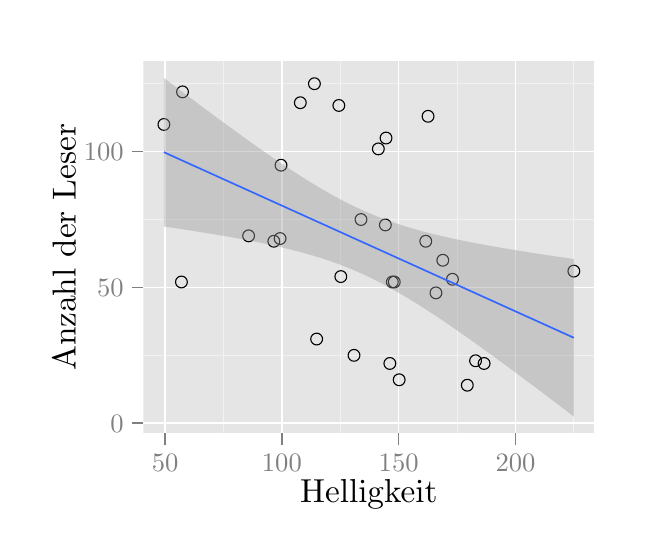
\begin{tikzpicture}[x=1pt,y=1pt]
\definecolor[named]{fillColor}{rgb}{1.00,1.00,1.00}
\path[use as bounding box,fill=fillColor,fill opacity=0.00] (0,0) rectangle (216.81,180.67);
\begin{scope}
\path[clip] (  0.00,  0.00) rectangle (216.81,180.67);
\definecolor[named]{drawColor}{rgb}{1.00,1.00,1.00}
\definecolor[named]{fillColor}{rgb}{1.00,1.00,1.00}

\path[draw=drawColor,line width= 0.6pt,line join=round,line cap=round,fill=fillColor] (  0.00,  0.00) rectangle (216.81,180.68);
\end{scope}
\begin{scope}
\path[clip] ( 41.82, 34.03) rectangle (204.77,168.63);
\definecolor[named]{fillColor}{rgb}{0.90,0.90,0.90}

\path[fill=fillColor] ( 41.82, 34.03) rectangle (204.77,168.63);
\definecolor[named]{drawColor}{rgb}{0.95,0.95,0.95}

\path[draw=drawColor,line width= 0.3pt,line join=round] ( 41.82, 62.27) --
	(204.77, 62.27);

\path[draw=drawColor,line width= 0.3pt,line join=round] ( 41.82,111.34) --
	(204.77,111.34);

\path[draw=drawColor,line width= 0.3pt,line join=round] ( 41.82,160.42) --
	(204.77,160.42);

\path[draw=drawColor,line width= 0.3pt,line join=round] ( 70.75, 34.03) --
	( 70.75,168.63);

\path[draw=drawColor,line width= 0.3pt,line join=round] (112.95, 34.03) --
	(112.95,168.63);

\path[draw=drawColor,line width= 0.3pt,line join=round] (155.15, 34.03) --
	(155.15,168.63);

\path[draw=drawColor,line width= 0.3pt,line join=round] (197.35, 34.03) --
	(197.35,168.63);
\definecolor[named]{drawColor}{rgb}{1.00,1.00,1.00}

\path[draw=drawColor,line width= 0.6pt,line join=round] ( 41.82, 37.73) --
	(204.77, 37.73);

\path[draw=drawColor,line width= 0.6pt,line join=round] ( 41.82, 86.81) --
	(204.77, 86.81);

\path[draw=drawColor,line width= 0.6pt,line join=round] ( 41.82,135.88) --
	(204.77,135.88);

\path[draw=drawColor,line width= 0.6pt,line join=round] ( 49.65, 34.03) --
	( 49.65,168.63);

\path[draw=drawColor,line width= 0.6pt,line join=round] ( 91.85, 34.03) --
	( 91.85,168.63);

\path[draw=drawColor,line width= 0.6pt,line join=round] (134.05, 34.03) --
	(134.05,168.63);

\path[draw=drawColor,line width= 0.6pt,line join=round] (176.25, 34.03) --
	(176.25,168.63);
\definecolor[named]{drawColor}{rgb}{0.00,0.00,0.00}

\path[draw=drawColor,line width= 0.4pt,line join=round,line cap=round] (150.00, 96.62) circle (  2.13);

\path[draw=drawColor,line width= 0.4pt,line join=round,line cap=round] (164.93, 59.33) circle (  2.13);

\path[draw=drawColor,line width= 0.4pt,line join=round,line cap=round] ( 91.21,104.47) circle (  2.13);

\path[draw=drawColor,line width= 0.4pt,line join=round,line cap=round] (129.24,109.38) circle (  2.13);

\path[draw=drawColor,line width= 0.4pt,line join=round,line cap=round] (158.86, 51.47) circle (  2.13);

\path[draw=drawColor,line width= 0.4pt,line join=round,line cap=round] (134.24, 53.44) circle (  2.13);

\path[draw=drawColor,line width= 0.4pt,line join=round,line cap=round] (161.84, 60.31) circle (  2.13);

\path[draw=drawColor,line width= 0.4pt,line join=round,line cap=round] (143.85,103.49) circle (  2.13);

\path[draw=drawColor,line width= 0.4pt,line join=round,line cap=round] (130.87, 59.33) circle (  2.13);

\path[draw=drawColor,line width= 0.4pt,line join=round,line cap=round] (147.53, 84.84) circle (  2.13);

\path[draw=drawColor,line width= 0.4pt,line join=round,line cap=round] (126.71,136.86) circle (  2.13);

\path[draw=drawColor,line width= 0.4pt,line join=round,line cap=round] (104.42, 68.16) circle (  2.13);

\path[draw=drawColor,line width= 0.4pt,line join=round,line cap=round] (131.77, 88.77) circle (  2.13);

\path[draw=drawColor,line width= 0.4pt,line join=round,line cap=round] (153.50, 89.75) circle (  2.13);

\path[draw=drawColor,line width= 0.4pt,line join=round,line cap=round] (120.44,111.34) circle (  2.13);

\path[draw=drawColor,line width= 0.4pt,line join=round,line cap=round] ( 98.52,153.55) circle (  2.13);

\path[draw=drawColor,line width= 0.4pt,line join=round,line cap=round] ( 79.83,105.45) circle (  2.13);

\path[draw=drawColor,line width= 0.4pt,line join=round,line cap=round] (197.36, 92.70) circle (  2.13);

\path[draw=drawColor,line width= 0.4pt,line join=round,line cap=round] (132.47, 88.77) circle (  2.13);

\path[draw=drawColor,line width= 0.4pt,line join=round,line cap=round] (103.61,160.42) circle (  2.13);

\path[draw=drawColor,line width= 0.4pt,line join=round,line cap=round] (112.44,152.56) circle (  2.13);

\path[draw=drawColor,line width= 0.4pt,line join=round,line cap=round] ( 88.95,103.49) circle (  2.13);

\path[draw=drawColor,line width= 0.4pt,line join=round,line cap=round] (117.92, 62.27) circle (  2.13);

\path[draw=drawColor,line width= 0.4pt,line join=round,line cap=round] ( 91.54,130.97) circle (  2.13);

\path[draw=drawColor,line width= 0.4pt,line join=round,line cap=round] (129.49,140.79) circle (  2.13);

\path[draw=drawColor,line width= 0.4pt,line join=round,line cap=round] ( 49.23,145.69) circle (  2.13);

\path[draw=drawColor,line width= 0.4pt,line join=round,line cap=round] ( 55.95,157.47) circle (  2.13);

\path[draw=drawColor,line width= 0.4pt,line join=round,line cap=round] ( 55.56, 88.77) circle (  2.13);

\path[draw=drawColor,line width= 0.4pt,line join=round,line cap=round] (113.15, 90.73) circle (  2.13);

\path[draw=drawColor,line width= 0.4pt,line join=round,line cap=round] (144.68,148.64) circle (  2.13);
\definecolor[named]{fillColor}{rgb}{0.60,0.60,0.60}

\path[fill=fillColor,fill opacity=0.40] ( 49.23,162.51) --
	( 51.10,161.09) --
	( 52.98,159.67) --
	( 54.85,158.26) --
	( 56.73,156.84) --
	( 58.60,155.43) --
	( 60.48,154.03) --
	( 62.35,152.63) --
	( 64.23,151.23) --
	( 66.10,149.84) --
	( 67.98,148.45) --
	( 69.85,147.07) --
	( 71.73,145.70) --
	( 73.60,144.33) --
	( 75.48,142.97) --
	( 77.35,141.62) --
	( 79.23,140.27) --
	( 81.10,138.93) --
	( 82.98,137.61) --
	( 84.85,136.29) --
	( 86.73,134.99) --
	( 88.60,133.69) --
	( 90.48,132.42) --
	( 92.35,131.15) --
	( 94.23,129.90) --
	( 96.10,128.67) --
	( 97.98,127.46) --
	( 99.85,126.27) --
	(101.73,125.10) --
	(103.60,123.95) --
	(105.48,122.83) --
	(107.35,121.74) --
	(109.23,120.67) --
	(111.10,119.63) --
	(112.98,118.63) --
	(114.85,117.65) --
	(116.73,116.71) --
	(118.60,115.81) --
	(120.48,114.94) --
	(122.35,114.11) --
	(124.23,113.31) --
	(126.10,112.54) --
	(127.98,111.81) --
	(129.86,111.11) --
	(131.73,110.44) --
	(133.61,109.81) --
	(135.48,109.20) --
	(137.36,108.62) --
	(139.23,108.06) --
	(141.11,107.53) --
	(142.98,107.02) --
	(144.86,106.53) --
	(146.73,106.06) --
	(148.61,105.61) --
	(150.48,105.17) --
	(152.36,104.75) --
	(154.23,104.34) --
	(156.11,103.95) --
	(157.98,103.56) --
	(159.86,103.19) --
	(161.73,102.83) --
	(163.61,102.47) --
	(165.48,102.13) --
	(167.36,101.79) --
	(169.23,101.46) --
	(171.11,101.13) --
	(172.98,100.82) --
	(174.86,100.50) --
	(176.73,100.20) --
	(178.61, 99.89) --
	(180.48, 99.60) --
	(182.36, 99.30) --
	(184.23, 99.01) --
	(186.11, 98.73) --
	(187.98, 98.45) --
	(189.86, 98.17) --
	(191.73, 97.89) --
	(193.61, 97.62) --
	(195.48, 97.35) --
	(197.36, 97.08) --
	(197.36, 40.15) --
	(195.48, 41.58) --
	(193.61, 43.01) --
	(191.73, 44.43) --
	(189.86, 45.85) --
	(187.98, 47.27) --
	(186.11, 48.69) --
	(184.23, 50.10) --
	(182.36, 51.51) --
	(180.48, 52.91) --
	(178.61, 54.31) --
	(176.73, 55.71) --
	(174.86, 57.10) --
	(172.98, 58.48) --
	(171.11, 59.86) --
	(169.23, 61.24) --
	(167.36, 62.60) --
	(165.48, 63.96) --
	(163.61, 65.31) --
	(161.73, 66.66) --
	(159.86, 67.99) --
	(157.98, 69.32) --
	(156.11, 70.63) --
	(154.23, 71.93) --
	(152.36, 73.22) --
	(150.48, 74.50) --
	(148.61, 75.76) --
	(146.73, 77.00) --
	(144.86, 78.23) --
	(142.98, 79.44) --
	(141.11, 80.63) --
	(139.23, 81.79) --
	(137.36, 82.93) --
	(135.48, 84.05) --
	(133.61, 85.14) --
	(131.73, 86.20) --
	(129.86, 87.23) --
	(127.98, 88.23) --
	(126.10, 89.20) --
	(124.23, 90.13) --
	(122.35, 91.03) --
	(120.48, 91.89) --
	(118.60, 92.72) --
	(116.73, 93.51) --
	(114.85, 94.27) --
	(112.98, 94.99) --
	(111.10, 95.68) --
	(109.23, 96.34) --
	(107.35, 96.98) --
	(105.48, 97.58) --
	(103.60, 98.15) --
	(101.73, 98.70) --
	( 99.85, 99.23) --
	( 97.98, 99.74) --
	( 96.10,100.22) --
	( 94.23,100.69) --
	( 92.35,101.14) --
	( 90.48,101.57) --
	( 88.60,101.99) --
	( 86.73,102.40) --
	( 84.85,102.79) --
	( 82.98,103.17) --
	( 81.10,103.54) --
	( 79.23,103.90) --
	( 77.35,104.26) --
	( 75.48,104.60) --
	( 73.60,104.94) --
	( 71.73,105.27) --
	( 69.85,105.59) --
	( 67.98,105.91) --
	( 66.10,106.22) --
	( 64.23,106.52) --
	( 62.35,106.82) --
	( 60.48,107.12) --
	( 58.60,107.41) --
	( 56.73,107.70) --
	( 54.85,107.99) --
	( 52.98,108.27) --
	( 51.10,108.55) --
	( 49.23,108.82) --
	cycle;
\definecolor[named]{drawColor}{rgb}{0.20,0.40,1.00}

\path[draw=drawColor,line width= 0.6pt,line join=round] ( 49.23,135.67) --
	( 51.10,134.82) --
	( 52.98,133.97) --
	( 54.85,133.12) --
	( 56.73,132.27) --
	( 58.60,131.42) --
	( 60.48,130.57) --
	( 62.35,129.73) --
	( 64.23,128.88) --
	( 66.10,128.03) --
	( 67.98,127.18) --
	( 69.85,126.33) --
	( 71.73,125.48) --
	( 73.60,124.63) --
	( 75.48,123.78) --
	( 77.35,122.94) --
	( 79.23,122.09) --
	( 81.10,121.24) --
	( 82.98,120.39) --
	( 84.85,119.54) --
	( 86.73,118.69) --
	( 88.60,117.84) --
	( 90.48,116.99) --
	( 92.35,116.15) --
	( 94.23,115.30) --
	( 96.10,114.45) --
	( 97.98,113.60) --
	( 99.85,112.75) --
	(101.73,111.90) --
	(103.60,111.05) --
	(105.48,110.20) --
	(107.35,109.36) --
	(109.23,108.51) --
	(111.10,107.66) --
	(112.98,106.81) --
	(114.85,105.96) --
	(116.73,105.11) --
	(118.60,104.26) --
	(120.48,103.41) --
	(122.35,102.57) --
	(124.23,101.72) --
	(126.10,100.87) --
	(127.98,100.02) --
	(129.86, 99.17) --
	(131.73, 98.32) --
	(133.61, 97.47) --
	(135.48, 96.62) --
	(137.36, 95.78) --
	(139.23, 94.93) --
	(141.11, 94.08) --
	(142.98, 93.23) --
	(144.86, 92.38) --
	(146.73, 91.53) --
	(148.61, 90.68) --
	(150.48, 89.83) --
	(152.36, 88.99) --
	(154.23, 88.14) --
	(156.11, 87.29) --
	(157.98, 86.44) --
	(159.86, 85.59) --
	(161.73, 84.74) --
	(163.61, 83.89) --
	(165.48, 83.04) --
	(167.36, 82.20) --
	(169.23, 81.35) --
	(171.11, 80.50) --
	(172.98, 79.65) --
	(174.86, 78.80) --
	(176.73, 77.95) --
	(178.61, 77.10) --
	(180.48, 76.25) --
	(182.36, 75.41) --
	(184.23, 74.56) --
	(186.11, 73.71) --
	(187.98, 72.86) --
	(189.86, 72.01) --
	(191.73, 71.16) --
	(193.61, 70.31) --
	(195.48, 69.46) --
	(197.36, 68.62);
\end{scope}
\begin{scope}
\path[clip] (  0.00,  0.00) rectangle (216.81,180.67);
\definecolor[named]{drawColor}{rgb}{0.50,0.50,0.50}

\node[text=drawColor,anchor=base east,inner sep=0pt, outer sep=0pt, scale=  0.96] at ( 34.71, 34.43) {0};

\node[text=drawColor,anchor=base east,inner sep=0pt, outer sep=0pt, scale=  0.96] at ( 34.71, 83.50) {50};

\node[text=drawColor,anchor=base east,inner sep=0pt, outer sep=0pt, scale=  0.96] at ( 34.71,132.57) {100};
\end{scope}
\begin{scope}
\path[clip] (  0.00,  0.00) rectangle (216.81,180.67);
\definecolor[named]{drawColor}{rgb}{0.50,0.50,0.50}

\path[draw=drawColor,line width= 0.6pt,line join=round] ( 37.55, 37.73) --
	( 41.82, 37.73);

\path[draw=drawColor,line width= 0.6pt,line join=round] ( 37.55, 86.81) --
	( 41.82, 86.81);

\path[draw=drawColor,line width= 0.6pt,line join=round] ( 37.55,135.88) --
	( 41.82,135.88);
\end{scope}
\begin{scope}
\path[clip] (  0.00,  0.00) rectangle (216.81,180.67);
\definecolor[named]{drawColor}{rgb}{0.50,0.50,0.50}

\path[draw=drawColor,line width= 0.6pt,line join=round] ( 49.65, 29.77) --
	( 49.65, 34.03);

\path[draw=drawColor,line width= 0.6pt,line join=round] ( 91.85, 29.77) --
	( 91.85, 34.03);

\path[draw=drawColor,line width= 0.6pt,line join=round] (134.05, 29.77) --
	(134.05, 34.03);

\path[draw=drawColor,line width= 0.6pt,line join=round] (176.25, 29.77) --
	(176.25, 34.03);
\end{scope}
\begin{scope}
\path[clip] (  0.00,  0.00) rectangle (216.81,180.67);
\definecolor[named]{drawColor}{rgb}{0.50,0.50,0.50}

\node[text=drawColor,anchor=base,inner sep=0pt, outer sep=0pt, scale=  0.96] at ( 49.65, 20.31) {50};

\node[text=drawColor,anchor=base,inner sep=0pt, outer sep=0pt, scale=  0.96] at ( 91.85, 20.31) {100};

\node[text=drawColor,anchor=base,inner sep=0pt, outer sep=0pt, scale=  0.96] at (134.05, 20.31) {150};

\node[text=drawColor,anchor=base,inner sep=0pt, outer sep=0pt, scale=  0.96] at (176.25, 20.31) {200};
\end{scope}
\begin{scope}
\path[clip] (  0.00,  0.00) rectangle (216.81,180.67);
\definecolor[named]{drawColor}{rgb}{0.00,0.00,0.00}

\node[text=drawColor,anchor=base,inner sep=0pt, outer sep=0pt, scale=  1.20] at (123.29,  9.03) {Helligkeit};
\end{scope}
\begin{scope}
\path[clip] (  0.00,  0.00) rectangle (216.81,180.67);
\definecolor[named]{drawColor}{rgb}{0.00,0.00,0.00}

\node[text=drawColor,rotate= 90.00,anchor=base,inner sep=0pt, outer sep=0pt, scale=  1.20] at ( 17.30,101.33) {Anzahl der Leser};
\end{scope}
\end{tikzpicture}

  \caption[Einfluss der Helligkeit auf Leser]{Einfluss der Helligkeit auf Leser}
\end{figure}

Das nächste wichtige Merkmal ist die Cover-Helligkeit eines Buchs.
Anders als beim Geschlecht der Hauptfigur, ist die Entstehung dieses
Merkmals ist nicht mehr direkt mit der Autorin oder dem Autor verbunden.
Das Cover wird zu einem Zeitpunkt, an dem die Geschichte schon längst an
einen Verlag verkauft worden ist, gestaltet. Es kann auch vorkommen,
dass das Cover bei neueren Fassungen komplett anders gestaltet wurde als
bei die Erstausgabe. Der Verlag hat schließlich die Aufgabe, die
Geschichte an den Endkunden zu verkaufen, das heißt, Kindern, deren
Eltern und weiteren potenziellen Käufern die Entscheidung zu
erleichtern.

Wir vermuten, dass die Verlage herausgefunden haben, dass dunkle
\emph{coole} Bücher Buben eher ansprechen als lieblich helle oder gar
rosa oder pastellfarbene Bücher. Der Verlag muss eine Entscheidung
treffen, für wen die Geschichte gedacht ist. Hier werden Inhalte eines
Buches von den dafür zuständigen Personen im Cover ausgedrückt und
gewissermaßen \emph{übersetzt}. Dabei wirkt es nicht überraschend, dass
sie sich an, in der Gesellschaft verfestigten Geschlechterrollenbildern
orientieren. Tatsächlich hat der \emph{Gender-Faktor} auf die Helligkeit
den größten Einfluss ($r=-0{,}51^{**}$). So ist die Helligkeit ein gutes
\emph{Transportmittel} um den Gender-Faktor ankommen zu
lassen.\footnote{Wir gehen davon aus, dass weitere Merkmale des Covers, die wir nicht operationalisiert haben, wie die Form der Darstellung oder die Komplexität des Bildes noch einen wesentlichen Anteil zur Übersetzung des Genderfaktor beitragen.}

Nicht übersehen darf man, dass nur das Leseverhalten von Buben von der
Helligkeit beeinflusst wird. Bei der Anzahl der Leserinnen kann kein
Zusammenhang mit der Helligkeit nachgewiesen werden. Das heißt Mädchen
lesen genauso helle wie dunkle Bücher. Buben meiden jedoch helle Bücher.
Auch das zeigt die Tendenz, dass Buben es eher vermeiden mädchenhafte
Literatur zu konsumieren, während der Spielraum der Mädchen hier weniger
eingeschränkt wird.

Betrachtet man die Bücher ohne die Vorlesebücher verringert sich der
Einfluss der Helligkeit. Für die Anzahl der Buben kann dann, durch die
Helligkeit keine signifikante Verbesserung des Modells erreicht werden.

\section{Buben bevorzugen Bücher für Ältere}

\begin{figure}
\center
  \label{alter}
  \small
% Created by tikzDevice version 0.6.2-92-0ad2792 on 2013-02-14 03:08:47
% !TEX encoding = UTF-8 Unicode
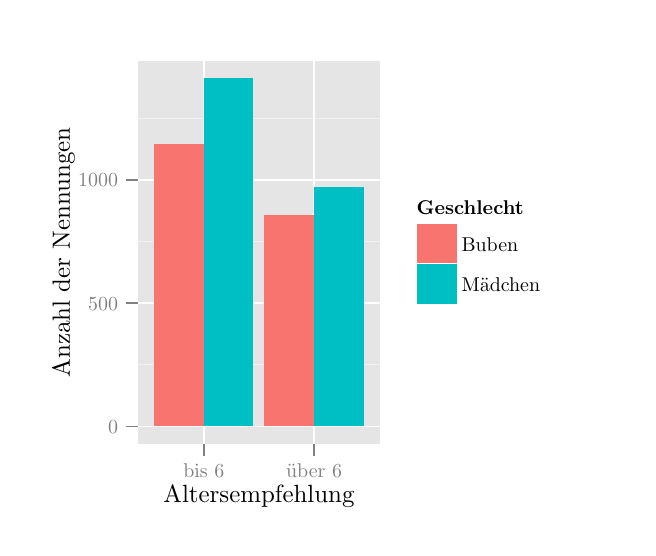
\begin{tikzpicture}[x=1pt,y=1pt]
\definecolor[named]{fillColor}{rgb}{1.00,1.00,1.00}
\path[use as bounding box,fill=fillColor,fill opacity=0.00] (0,0) rectangle (216.81,180.67);
\begin{scope}
\path[clip] (  0.00,  0.00) rectangle (216.81,180.67);
\definecolor[named]{drawColor}{rgb}{1.00,1.00,1.00}
\definecolor[named]{fillColor}{rgb}{1.00,1.00,1.00}

\path[draw=drawColor,line width= 0.6pt,line join=round,line cap=round,fill=fillColor] (  0.00,  0.00) rectangle (216.81,180.67);
\end{scope}
\begin{scope}
\path[clip] ( 39.75, 30.32) rectangle (127.38,168.63);
\definecolor[named]{fillColor}{rgb}{0.90,0.90,0.90}

\path[fill=fillColor] ( 39.75, 30.32) rectangle (127.38,168.63);
\definecolor[named]{drawColor}{rgb}{0.95,0.95,0.95}

\path[draw=drawColor,line width= 0.3pt,line join=round] ( 39.75, 58.87) --
	(127.38, 58.87);

\path[draw=drawColor,line width= 0.3pt,line join=round] ( 39.75,103.39) --
	(127.38,103.39);

\path[draw=drawColor,line width= 0.3pt,line join=round] ( 39.75,147.92) --
	(127.38,147.92);
\definecolor[named]{drawColor}{rgb}{1.00,1.00,1.00}

\path[draw=drawColor,line width= 0.6pt,line join=round] ( 39.75, 36.60) --
	(127.38, 36.60);

\path[draw=drawColor,line width= 0.6pt,line join=round] ( 39.75, 81.13) --
	(127.38, 81.13);

\path[draw=drawColor,line width= 0.6pt,line join=round] ( 39.75,125.65) --
	(127.38,125.65);

\path[draw=drawColor,line width= 0.6pt,line join=round] ( 63.65, 30.32) --
	( 63.65,168.63);

\path[draw=drawColor,line width= 0.6pt,line join=round] (103.48, 30.32) --
	(103.48,168.63);
\definecolor[named]{fillColor}{rgb}{0.97,0.46,0.43}

\path[fill=fillColor] ( 45.73, 36.60) rectangle ( 63.65,138.74);
\definecolor[named]{fillColor}{rgb}{0.00,0.75,0.77}

\path[fill=fillColor] ( 63.65, 36.60) rectangle ( 81.58,162.34);
\definecolor[named]{fillColor}{rgb}{0.97,0.46,0.43}

\path[fill=fillColor] ( 85.56, 36.60) rectangle (103.48,113.01);
\definecolor[named]{fillColor}{rgb}{0.00,0.75,0.77}

\path[fill=fillColor] (103.48, 36.60) rectangle (121.41,123.16);
\end{scope}
\begin{scope}
\path[clip] (  0.00,  0.00) rectangle (216.81,180.67);
\definecolor[named]{drawColor}{rgb}{0.50,0.50,0.50}

\node[text=drawColor,anchor=base east,inner sep=0pt, outer sep=0pt, scale=  0.72] at ( 32.64, 34.12) {0};

\node[text=drawColor,anchor=base east,inner sep=0pt, outer sep=0pt, scale=  0.72] at ( 32.64, 78.65) {500};

\node[text=drawColor,anchor=base east,inner sep=0pt, outer sep=0pt, scale=  0.72] at ( 32.64,123.17) {1000};
\end{scope}
\begin{scope}
\path[clip] (  0.00,  0.00) rectangle (216.81,180.67);
\definecolor[named]{drawColor}{rgb}{0.50,0.50,0.50}

\path[draw=drawColor,line width= 0.6pt,line join=round] ( 35.49, 36.60) --
	( 39.75, 36.60);

\path[draw=drawColor,line width= 0.6pt,line join=round] ( 35.49, 81.13) --
	( 39.75, 81.13);

\path[draw=drawColor,line width= 0.6pt,line join=round] ( 35.49,125.65) --
	( 39.75,125.65);
\end{scope}
\begin{scope}
\path[clip] (  0.00,  0.00) rectangle (216.81,180.67);
\definecolor[named]{drawColor}{rgb}{0.50,0.50,0.50}

\path[draw=drawColor,line width= 0.6pt,line join=round] ( 63.65, 26.05) --
	( 63.65, 30.32);

\path[draw=drawColor,line width= 0.6pt,line join=round] (103.48, 26.05) --
	(103.48, 30.32);
\end{scope}
\begin{scope}
\path[clip] (  0.00,  0.00) rectangle (216.81,180.67);
\definecolor[named]{drawColor}{rgb}{0.50,0.50,0.50}

\node[text=drawColor,anchor=base,inner sep=0pt, outer sep=0pt, scale=  0.72] at ( 63.65, 18.24) {bis 6};

\node[text=drawColor,anchor=base,inner sep=0pt, outer sep=0pt, scale=  0.72] at (103.48, 18.24) {über 6};
\end{scope}
\begin{scope}
\path[clip] (  0.00,  0.00) rectangle (216.81,180.67);
\definecolor[named]{drawColor}{rgb}{0.00,0.00,0.00}

\node[text=drawColor,anchor=base,inner sep=0pt, outer sep=0pt, scale=  0.90] at ( 83.57,  9.03) {Altersempfehlung};
\end{scope}
\begin{scope}
\path[clip] (  0.00,  0.00) rectangle (216.81,180.67);
\definecolor[named]{drawColor}{rgb}{0.00,0.00,0.00}

\node[text=drawColor,rotate= 90.00,anchor=base,inner sep=0pt, outer sep=0pt, scale=  0.90] at ( 15.23, 99.47) {Anzahl der Nennungen};
\end{scope}
\begin{scope}
\path[clip] (  0.00,  0.00) rectangle (216.81,180.67);
\definecolor[named]{fillColor}{rgb}{1.00,1.00,1.00}

\path[fill=fillColor] (136.25, 76.46) rectangle (195.90,122.49);
\end{scope}
\begin{scope}
\path[clip] (  0.00,  0.00) rectangle (216.81,180.67);
\definecolor[named]{drawColor}{rgb}{0.00,0.00,0.00}

\node[text=drawColor,anchor=base west,inner sep=0pt, outer sep=0pt, scale=  0.72] at (140.52,113.25) {\bfseries Geschlecht};
\end{scope}
\begin{scope}
\path[clip] (  0.00,  0.00) rectangle (216.81,180.67);
\definecolor[named]{drawColor}{rgb}{1.00,1.00,1.00}
\definecolor[named]{fillColor}{rgb}{0.95,0.95,0.95}

\path[draw=drawColor,line width= 0.6pt,line join=round,line cap=round,fill=fillColor] (140.52, 95.18) rectangle (154.97,109.64);
\end{scope}
\begin{scope}
\path[clip] (  0.00,  0.00) rectangle (216.81,180.67);
\definecolor[named]{fillColor}{rgb}{0.97,0.46,0.43}

\path[fill=fillColor] (140.52, 95.18) rectangle (154.97,109.64);

\path[] (140.52, 95.18) --
	(154.97,109.64);
\end{scope}
\begin{scope}
\path[clip] (  0.00,  0.00) rectangle (216.81,180.67);
\definecolor[named]{drawColor}{rgb}{1.00,1.00,1.00}
\definecolor[named]{fillColor}{rgb}{0.95,0.95,0.95}

\path[draw=drawColor,line width= 0.6pt,line join=round,line cap=round,fill=fillColor] (140.52, 80.73) rectangle (154.97, 95.18);
\end{scope}
\begin{scope}
\path[clip] (  0.00,  0.00) rectangle (216.81,180.67);
\definecolor[named]{fillColor}{rgb}{0.00,0.75,0.77}

\path[fill=fillColor] (140.52, 80.73) rectangle (154.97, 95.18);

\path[] (140.52, 80.73) --
	(154.97, 95.18);
\end{scope}
\begin{scope}
\path[clip] (  0.00,  0.00) rectangle (216.81,180.67);
\definecolor[named]{drawColor}{rgb}{0.00,0.00,0.00}

\node[text=drawColor,anchor=base west,inner sep=0pt, outer sep=0pt, scale=  0.72] at (156.78, 99.93) {Buben};
\end{scope}
\begin{scope}
\path[clip] (  0.00,  0.00) rectangle (216.81,180.67);
\definecolor[named]{drawColor}{rgb}{0.00,0.00,0.00}

\node[text=drawColor,anchor=base west,inner sep=0pt, outer sep=0pt, scale=  0.72] at (156.78, 85.48) {Mädchen};
\end{scope}
\end{tikzpicture}

  \caption[Einfluss von Altersempfehlung]{Einfluss von Altersempfehlung auf Leserinnen und Leser}
\end{figure}

Ein weiterer Einfluss auf das Leseverhalten, speziell von Buben, ist die
Dicke eines Buchs, beziehungsweise das eng damit zusammenhängende
empfohlene Alter. Und zwar steigt mit der Dicke der Bücher auch die
Anzahl der männlichen Leser. Auf den ersten Blick widerspricht dieser
Fakt den Ergebnissen der Lesesozialisationsforschung, in der Buben meist
als \emph{Lesemuffel} dargestellt werden. Vor allem, weil das
Leseverhalten von Mädchen dadurch nicht nachweisbar beeinflusst wird.

Um das Wirken der Dicke/des Alters haben wir zwei Vermutungen. Die erste
bezieht sich darauf, dass Mädchen früher zu lesen beginnen. Wir haben
die Kinder gefragt, welche Bücher sie gelesen haben. Die befragten
Kinder waren zwischen 8 und 10 Jahren und es ist durchaus vorstellbar,
dass die Mädchen früher zum Lesen von \emph{Geschichten-Büchern}
anfangen. Das heißt, dass sie davor weniger oder andere von uns nicht
untersuchte Bücher, wie die bei den Buben sehr beliebten Sachbücher,
lesen.

Die zweite Vermutung bezieht sich auf den \emph{Coolness-Faktor}. Das
heißt, dass es für Buben wichtiger ist, \emph{cool} zu sein. So kann
sich von unserer Forschungsgruppe ein männliches Mitglied noch sehr gut
erinnern, dass das empfohlene Alter auf den Büchern, für ihn, gerade im
Alter der Untersuchten, sehr wichtig war.

Wie man an Abb. \ref{alter} sieht, gibt es bei der durchschnittlichen
Anzahl an Lesern einen Unterschied zwischen Vorlesebücher und dem Rest,
bei der Anzahl der Leserinnen nicht. Ohne die Vorlesebücher hat die
Dicke im Modell keinen Einfluss mehr auf das Leseverhalten.

\section{Mädchen bevorzugen Bücher mit wenig Figuren am Cover}

Somit bleibt von den bis jetzt angesprochen Merkmalen nur mehr die
Anzahl der Figuren am Cover. Es besteht ein negativer linearer
Zusammenhang zwischen der Häufigkeit der Leserinnen und der Anzahl der
Figuren am Cover. Das heißt, je weniger Figuren am Cover sind, umso
höher ist die Wahrscheinlichkeit, dass das Buch von einem Mädchen
gelesen wurde.

Um zu verstehen, wie es zu diesem Merkmal kommt, ist es wieder sinnvoll
die Entstehung dieses Merkmals genauer zu beleuchten. Dieses Merkmal
entsteht, wie auch schon die Helligkeit, ohne den direkten Einfluss der
Verfasserin bzw. des Verfassers. Die Grafikabteilung des Verlags,
übersetzt hier wieder Inhalt in Design. Wobei wir vermuten, dass zwei
Aspekte der Geschichte für die Anzahl der Figuren wichtig sind.
Einerseits halten wir es für entscheidend, ob es sich um einen
Multiprotagonisten handelt, wie z.B bei der \emph{Knickerbockerbande}
oder den \emph{Wilden Hühnern}. Andererseits glauben wir, dass die Ebene
auf der die Geschichte stattfindet, ob es viel \emph{Psychologisches}
also z.B. einen \emph{Inneren Monolog} gibt, oder ob sich die meisten
Probleme auf soziales Handeln beziehen. Diese These wird auch davon
gestützt, dass die stärkste Korrelation der Anzahl der Figuren von dem
Merkmal \emph{Innerer Monolog} ausgeht ($r=0{,}36^\circ$).

Der Einfluss der Anzahl der Figuren am Cover verändert sich nicht, wenn
die Vorlesebücher ausgeschlossen werden.

\section{Zusammenfassung}

Abschließend lässt sich sagen, dass, egal ob es ein Vorlesebuch oder ein
Buch für junge Erwachsene ist, wenn im Titel ein weiblicher Name
vorkommt, das Buch eindeutig von mehr Mädchen als Buben gelesen wird.
Dieser Faktor motiviert Mädchen ein Buch zu kaufen und schreckt Buben
ab. Ein weiterer Punkt ist die Helligkeit. Helle Farben schrecken Buben
ab. Auf Mädchen hat die Helligkeit keinen Einfluss. Dafür lassen sich
Mädchen von der Anzahl der Figuren am Cover stark beeinflussen. Je mehr
Figuren am Cover sichtbar sind, desto eher lassen sie das Lesen des
Buchs bleiben. Des weiteren konnten wir bestätigen, dass Buben bei
Geschichtenbüchern eher zu Bücher für Ältere tendieren, wobei Mädchen
hier keinen Unterschied machen. Unsere Vermutung, dass man ein Buch
nicht aufzumachen braucht um herauszufinden, ob es eher Mädchen oder
Buben lesen, hat sich bestätigt.

\chapter{Fazit}

Das Ziel dieser Arbeit war die Beantwortung der Frage, ob und wie sich
Mädchen- und Bubenbücher inhaltlich und oberflächlich voneinander
unterscheiden. Wir konnten zeigen, dass es eindeutige Unterschiede im
Leseverhalten von Mädchen und Buben gibt, einige Werke können
tatsächlich als Mädchen- und Bubenbücher bezeichnet werden, wobei sich
Mädchenbücher hauptsächlich dadurch auszeichnen, dass Buben diese eben
nicht konsumieren. Dieses Ergebnis zieht sich beinahe durch die gesamte
Untersuchung und bestätigt die Vermutung, dass Mädchen und Frauen einen
größeren Spielraum in ihren Handlungen und Eigenschaften haben, während
Buben und Männer weibliche und feminine Bereiche eher meiden, als das
umgekehrt der Fall zu sein scheint.

Außerdem konsumieren die kindlichen Leser häufig Bücher, in denen die
Hauptfiguren dasselbe Geschlecht wie sie selbst haben. Dass Hauptfiguren
oft anti- klischeehafte Verhaltensweisen und Einstellungen haben, war
anzunehmen, da viele Autor\_innen bemüht waren und sind, Stereotype
aufzubrechen und differenzierte Geschlechterrollenbilder zu entwerfen.
Bücher werden nicht nur geschrieben, um bestehende reale Verhältnisse
abzubilden, sondern auch um zu verändern. Nichtsdestotrotz fanden wir
gerade in Werken, die eher von Buben konsumiert werden, eine Hauptfigur
mit maskulinen Eigenschaften. In den beliebtesten Mädchenbüchern konnten
wir sowohl maskuline als auch feminine Protagonisten identifizieren.

Ein weiteres deutliches Ergebnis ist, dass Alltagsgeschichten
hauptsächlich von Mädchen gelesen werden und Buben vor allem zu
Abenteuergeschichten greifen. Einblicke in die Gefühlswelt und das
Selbstbild der Protagonisten, kommen in den von uns analysierten
Alltags-Büchern vor, während das Lösen von Aufgaben und Rätseln ein
wichtiges Element in Abenteuergeschichten bildet.

Ebenso konnten wir zeigen, dass man von den oberflächlichen Merkmalen
eines Buches, schnell auf das Geschlecht der Lesenden schließen kann.
Natürlich verfolgen Verlage mit dem Design des Buchumschlags genau
dieses Ziel, Marketing lebt schließlich von der Bildung von
Käufergruppen.

Fruchtbar wäre eine Studie, die eine größere Bandbreite an Büchern
abdeckt und auch das Rezeptionsverhalten der Kinder zu untersuchen
versucht. Diese eher psychologisch motivierte Vorgehensweise, könnte
nützlich sein, um den Einfluss von Medien auf das Verhalten von ihren
Rezipient\_innen festzustellen. Bei der Vielfalt an Angeboten für Kinder
in jedem Alter, wäre es vielleicht übertrieben anzunehmen, dass ein paar
Bücher das Geschlechtsrollenbild von Kindern maßgeblich beeinflussen
können, allerdings können bestimmte Vorbilder, die hier die
Protagonisten der Bücher sind, viel über eine Gesellschaft aussagen.
